\documentclass[10pt]{beamer}
\usepackage[english]{babel}
\setbeamerfont{structure}{family=\rmfamily} 

\let\proof\relax
\let\endproof\relax
\let\qed\relax
\usepackage{amsthm}

\usepackage{graphicx}
\usepackage{graphics}
\usepackage{hyperref}
\usepackage{mathtools}
%\usepackage{coqdoc}
\usepackage{amsmath}
\usepackage{amssymb}
\usepackage[makeroom]{cancel}
\usepackage{xcolor}
\beamertemplatenavigationsymbolsempty
\setbeamertemplate{blocks}[rounded][shadow=true]
\setbeamertemplate{bibliography item}[text]
\setbeamertemplate{caption}[numbered]
\usetheme{default} 
\usecolortheme{seahorse}
\mode<presentation>
{
   \setbeamercovered{transparent}
   \setbeamertemplate{items}[ball]
   \setbeamertemplate{theorems}[numbered]
   \setbeamertemplate{footline}[frame number]

}

% structured proofs a la Leslie Lamport 
\usepackage{pf2}

% slides for sections and subsections
\AtBeginSection{\frame{\sectionpage}}
\AtBeginSubsection{\frame{\subsectionpage}}

\begin{document}
\newtheorem{mydef}{Definition}
\newtheorem{notation}{Notation}
\newtheorem{lem}{Lemma}
\newtheorem{theo}{Theorem}
\newtheorem{col}{Colollary}
\newtheorem{com}{Comment}
\newtheorem{exa}{Example}

% alternative definitions you may use if you want
\newtheorem{remark}{Remark}




\title {Topics on Hindley's Simple Type Theory*: 8E and 8F}

\author[Francisca Cappellesso and Gabriel Silva]{\small {Francisca Cappellesso \& Gabriel Silva}}
\institute{* - Presentation adapted from the work of Thiago Mendonça and Washington Ribeiro \\
% commented by KK (put image if you want)
%\includegraphics[scale=.08]{Amrita.jpg}\medskip\\ 
\sc{Type Theory Class - 1/2020 - Universidade de Bras\'{i}lia - UnB} \\  
}

\date{\small June 22, 2020} 
%--------------------------------------------------------------------------%
\begin{frame}
\titlepage
\end{frame}
%---------------------------------------------------------------------------%
\begin{frame}{Outline of Presentation}
    \setbeamertemplate{section in toc}[sections numbered]
    %\setcounter{tocdepth}{1}
    \tableofcontents
\end{frame}

%---------------------------------------------------------------------------

% this is the part of the presentation done by thiago and washington, ok? 
% by uncommenting the line below you can see the presentation they did. 
% \section{Motivation}

\begin{frame}{Motivation}

\begin{itemize}
 \item Given a type $\tau$, how many \textbf{closed} terms can recive $\tau$ in TA$_{\lambda}$?\\[0.5cm]
 \item How many are in a $\beta$-normal form?\\[0.5cm]
 \item The algorithm of Ben-Yelles (1979) answers the 'how many' question for closed $\beta$-normal forms\\[0.5cm]
 \item By the Curry-Howard correspondence, we will have a decision procedure for the Intuitionist Implicational Logic 
\end{itemize}


 
\end{frame}

\section{Inhabitants}

\begin{frame}{Inhabitants classes}

\begin{mydef}[Inhabitants]
\begin{itemize}
 \item \textbf{untyped inhabitant}: closed $M$ such that $\vdash_{\lambda} M : \tau$
 \item \textbf{typed inhabitant}: closed $M^{\tau}$
\end{itemize}
\end{mydef}

\begin{itemize} 
 \item[(i)]  \textbf{\textit{Habs}$_u(\tau)$}: untyped inhabitants
 \item[(ii)] \textbf{\textit{Habs}$_t(\tau)$}: typed inhabitants
 \item[(iii)]\textbf{\textit{Nhabs}$_u(\tau)$}: untyped inhabitants in a $\beta$-normal form
 \item[(iv)]\textbf{\textit{Nhabs}$_t(\tau)$}: typed inhabitants in a $\beta$-normal form
 \item[(v)]\textbf{\textit{Nhabs}$_{\eta}(\tau)$}: typed $\beta\eta$-normal inhabitants
 \item[(vi)]\textbf{\textit{Princ}$(\tau)$}: principal inhabitants
 \item[(vii)]\textbf{\textit{Nprinc}$(\tau)$}: principal inhabitants in a $\beta$-normal form
 \item[(viii)]\textbf{\textit{Nprinc}$_{\eta}(\tau)$}: principal inhabitants in a $\beta\eta$-normal form
\end{itemize}

\end{frame}

\begin{frame}{Typed $\beta$-nf's}

\begin{lem}[Structure of a typed $\beta$-nf]\label{8A5}
 Let $\Gamma$ be a type context. Every $\beta$-nf $N^{\alpha} \in \mathbb{TT}(\Gamma)$ can be expressed uniquely in the form:\\[0.3 cm]
 
\begin{itemize}
 \item[(i)] ($\lambda x_1^{\tau_1} ... \,x_m^{\tau_m} \, . \,
   (v^{(\rho_1 \rightarrow \cdots \rho_n \rightarrow \tau^*)} M^{\rho_1}_1 \cdots
   M^{\rho_n}_n)^{\tau^*})^{(\tau_1 \rightarrow \cdots \tau_m \rightarrow \tau^*)}$ \\where $m \geq 0$, $n \geq 0$, and\\[0.3 cm]
   

 \item[(ii)] $ \tau \equiv \tau_1 \rightarrow \cdots \tau_m \rightarrow \tau^*$ \\ for some $\tau^*$, possibly composite, and \\[0.3 cm]
 

 \item[(iii)] each $M^{\rho_j}_j$ is a $\beta$-nf that is typed relative to  $\Gamma \cup \{x_1 : \tau_1,\cdots, x_m : \tau_m\}$
\end{itemize}
\end{lem}

\end{frame}


\begin{frame}{Typed $\beta$-nf's}
\begin{proof}[Induction in $N^{\cancel{\alpha}}$:]
\begin{itemize}
 \item[(IB)] : $N^{\alpha} \equiv x^{\alpha}$, $x$ is in $\beta$-nf and $x \in \mathbb{TT}(\Gamma)$
 \item[(Case 1)] : $N^{\cancel{\alpha}} \equiv A B$
 
 $A$ is not an abstraction because if it was, $A B$ would not be in $\beta$-nf. 
 $A \equiv v H_1 \cdots H_k$. And by IH $A^{\gamma \rightarrow \alpha} \in \mathbb{TT}(\Gamma_1)$ and $B^{\gamma} \in \mathbb{TT}(\Gamma_2)$. 
 
 So using $\alpha$ equivalence to avoid clashes,
 
 $N^{\alpha} \in \mathbb{TT}(\Gamma_1 \cup \Gamma_2)$ is in the form
 $(v^{\rho_1\rightarrow \cdots \rho_k \rightarrow \gamma \rightarrow \alpha} H^{\rho_1}_1 \cdots
 H^{\rho_k}_k B^{\gamma})^{\alpha}$
 
 \item[(Case 2)] : $N^{\cancel{\alpha}} \equiv \lambda x \, . \, A$
 
 By IH, $A^{\gamma} \in \mathbb{TT}(\Gamma_1)$ and
it has the anounced form. 

Thus, $(\lambda x^{\omega}\, . \,
A^{\gamma})^{\omega \rightarrow \gamma} \in \mathbb{TT}(\Gamma_1 - \{x:
\omega\})$ has the same form.
\end{itemize} 
\end{proof}
\end{frame}



\begin{frame}{Long $\beta$-nf's}

 \begin{mydef}[Long $\beta$-nf's]
The $\beta$-nf $M^{\tau}$ is \textbf{long} or \textbf{maximal} 
iff each component with form ($z\, P_1 \cdots P_n)(n \geq 0)$ that is
not in a function position has atomic type.
\end{mydef}
\vspace*{0.3cm}

\begin{notation}[$Long(\tau)$]
 long normal inhabitants of $\tau$ (typed or untyped)
\end{notation}
\vspace*{0.3cm}

\begin{exa}[$\tau \equiv ((a \to b) \to c) \to (a \to b) \to c$]
\begin{itemize}
 \item[(i)] $M^{\tau} \equiv \lambda x^{(a\to b) \to c} \, y^{a \to b} \cdot x^{(a \to b) \to c} \, y^{a \to b}$ 
 \item[(ii)] $N^{\tau} \equiv \lambda x^{(a\to b) \to c} \, y^{a \to b} \cdot x^{(a \to b) \to c} \, (\lambda z \cdot y^{a \to b}\, z^a)$ \checkmark
\end{itemize}
\end{exa}

\end{frame}

\begin{frame}{Long $\beta$-nf's} 
 \begin{lem}[Completeness of $Long(\tau)$] \label{8A8} Every normal inhabitant of $\tau$ can be $\eta$-expanded to a long normal inhabitant of $\tau$.
And this long inhabitant is unique (modulo $\equiv_{\alpha}$); ie
\begin{center}
$\{M^{\tau}, N^{\tau} \in \mbox{Long}(\tau) \mbox{ and } M^{\tau} =_{\eta} N^{\tau}\} \Longrightarrow  M^{\tau} \equiv_{\alpha} N^{\tau}$ 
\end{center}
In particular
\begin{center}
 Nhabs$(\tau) = \emptyset \Longleftrightarrow$ Long$(\tau) = \emptyset$. 
\end{center}


\end{lem}

\begin{figure}[h]
   \centering
   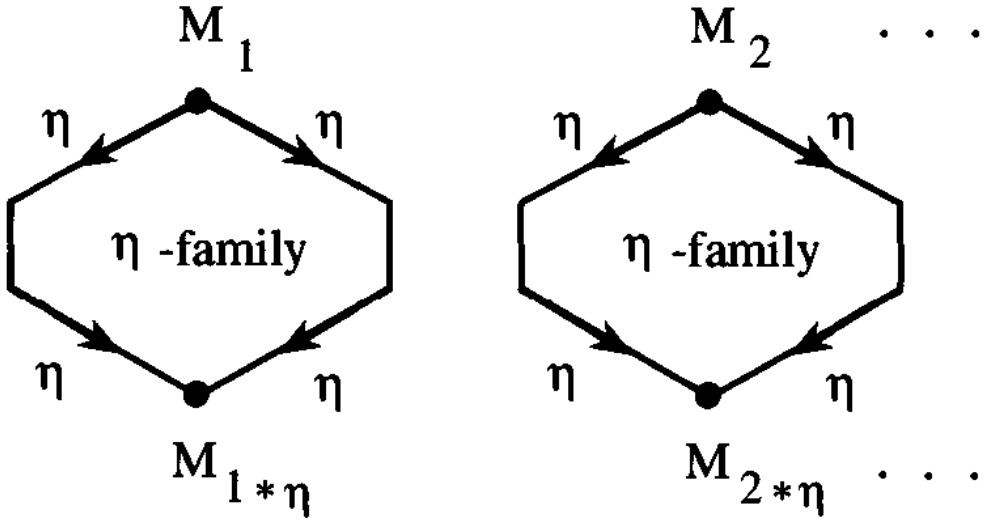
\includegraphics[scale=0.3]{fig1.png}
\end{figure}
\end{frame}

\begin{frame}{Long $\beta$-nf's}


\begin{proof}
 \begin{itemize}
  \item Let $P^{\tau} \in Nhabs(\tau)$
  \item $\eta$-expand $P^{\tau}$ to $P^{\tau +} \in Long(\tau)$. We must show that $P^{\tau +}$ is unique
  \begin{center}
   $M^{\tau} \in Long(\tau), \,\,\, M^{\tau}\twoheadrightarrow_{\eta} P^{\tau} \,\,\,\,\Longrightarrow \,\,\,\,M^{\tau} \equiv_{\alpha} P^{\tau +}$
  \end{center}
  \item suppose $P^{\tau}$ contains a component $(y\,Q_1\cdots Q_n)^{\sigma}$ that is not long
  \item it is not in function position and $\sigma \equiv \sigma_1 \to \cdots \to \sigma_k \to a\,\,\,\,\, (k \geq 1)$ 
  \item given new variables $z_1, ..., z_k$ not occuring in $P^{\cancel{\tau}}$, replace this component by
  \begin{center}
   $(\lambda z_1^{\sigma_1}\,...\, z_k^{\sigma_k} \cdot ((y\,Q_1\cdots Q_n)^{\sigma}\, z_1^{\sigma_1}\cdots z_k^{\sigma_k})^a)^{\sigma}$
  \end{center}
  \item[(i)] Make similar replacements until there are no short components in $P^{\tau}$. Call the result $P^{\tau +}$
  \item[(ii)] this replacements are $\eta$-expansions and its result is still a $\beta$-nf
  \item[(iii)] the proof is complete with rotine induction in $|P^{\tau}|$
 \end{itemize}
\end{proof}

\end{frame}

\begin{frame}{Long $\beta$-nf's}
 \begin{itemize}
  \item[(i)] Each replacement may introduce new short components with types $\sigma_1, ..., \sigma_k$, but these types are shorter than $\sigma$ so
   the replacement process will terminate\\[0.3cm]
  \item[(ii)] in $(\lambda z_1^{\sigma_1}\,...\, z_k^{\sigma_k} \cdot ((y\,Q_1\cdots Q_n)^{\sigma}\, z_1^{\sigma_1}\cdots z_k^{\sigma_k})^a)^{\sigma}$ the 
              $\beta$-reductions could ocurr just inside $Q_1\cdots Q_n$, but it is contraditory with the fact that $(y\,Q_1\cdots Q_n)^{\sigma}$ is $\beta$-nf\\[0.3cm]
  \item[(iii)] Now the induction over $|P^{\tau} \equiv \lambda x_1^{\tau_1} ... \,x_m^{\tau_m} \, . \, v\, M^{\rho_1}_1 \cdots M^{\rho_n}_n|$:\\[0.2 cm]
     \begin{itemize}
      \item By IH, for each $j$, $Long(\tau)\,\,\, \mbox{\reflectbox{$\in$}} \,\,\,M_j^{\rho_j +} \!\! \twoheadrightarrow_{\eta} \!M_j^{\rho_j}$ and $M_j^{\rho_j +}$ is unique\\[0.3 cm]
      \item $P^{\tau +} \equiv \lambda x_1^{\tau_1} ... \,x_m^{\tau_m} \, z_1^{\sigma_1}\,...\, z_k^{\sigma_k} . \, v\, M^{\rho_1 +}_1 \cdots M^{\rho_n +}_n \, z_1^{\sigma_1}\,...\, z_k^{\sigma_k}$\\[0.3 cm]
      \item $P^{\tau +} \in Long(\tau), \,\,\, P^{\tau +}\twoheadrightarrow_{\eta} P^{\tau}$\\[0.3 cm]
      \item $M^{\tau} \in Long(\tau), \,\,\, M^{\tau}\twoheadrightarrow_{\eta} P^{\tau} \,\,\,\,\Longrightarrow \,\,\,\,M^{\tau} \equiv_{\alpha} P^{\tau +}$\\
     \end{itemize}
 \end{itemize}

\end{frame}



\begin{frame}
 
 \begin{mydef}[Cardinality of $\mathbb{S}$]
 The number of members (modulo $\equiv_{\alpha}$) of a set $\mathbb{S}$.
 \begin{itemize}
  \item $\#(Nhabs(\tau))  \longleftrightarrow  \#(\tau)$
  \item $\#(Nhabs_{\eta}(\tau)) \longleftrightarrow \#_{\eta}(\tau)$
 \end{itemize}
\end{mydef}
 
 \begin{notation}
  $\{M^{\tau}\}_\eta \equiv$ the set of all terms that $\eta$-reduces from $M^{\tau}$ 
  \end{notation}

\begin{lem}\label{8A10}

    \begin{itemize}


           \item[(i)] The $\eta$-families  $\{M^{\tau}\}_\eta$ of long typed terms $M^{\tau}$ 
             patitions $Nhabs(\tau)$ into non-overlapping finite subsets. Each $\eta$-family contain one long
             member and one $\beta \eta$-nf.

        \item[(ii)] $\#_{\eta}(\tau) = \#(Long(\tau))$
        
        \item[(iii)] $\#(\tau)$ is infinte, finite or zero according to 
         
         $\#_\eta(\tau)$ is infinite, finite or zero.

      \end{itemize}
\end{lem}

\end{frame}

\begin{frame}

\begin{proof}
 \begin{itemize}
  \item $M^{\tau} \in \mathbb{TT}(\Gamma), \,\,\,\{M^{\tau}\}_{\eta}$ is finite (by the lemma \textbf{CR}$_{\eta}$) 
  \item $\{M^{\tau}\}_{\eta} \subseteq \mathbb{TT}(\Gamma)$ (lemma \textbf{5B7.1})
  \item if $M^{\tau}$ is a $\beta$-nf then so are all members of $\{M^{\tau}\}$ (typed analogue of the lemma \textbf{1C9.3})
 \begin{center}
  $M^{\tau} \in Nhabs(\tau) \,\,\,\Longrightarrow \,\,\,\{M^{\tau}\}_{\eta} \subseteq Nhabs(\tau)$
 \end{center}
  \item if $M^{\tau}$ is a $\beta$-nf its $\eta$-family contains exactly one $\beta\eta$-nf (typed analogue of the lemma \textbf{1C9.3})
  \item each normal inhabitant of $\tau$ is in the $\eta$-family of exactly one long normal inhabitant (by the lemma \ref{8A8})
  \item And by the \textbf{WN} lemma, $\#(\tau)$ is infinte, finite or zero according to  $\#_\eta(\tau)$ is infinite, finite or zero.
 \end{itemize}
 \end{proof}
 
 
\end{frame}


\begin{frame}
 \begin{lem}
    Let $M^{\tau+}$ be the unique member of $Long(\tau)$ to which
    $M^{\tau}$ $\eta$-expands. 

  \begin{center}
       $M^{\tau} \in Nprinc(\tau) \Longrightarrow M^{\tau+} \in Nprinc(\tau)$
   \end{center}
\end{lem}

\begin{proof}
\begin{itemize}
  \item $\eta$-expansion in the lemma \ref{8A8} preserves principality
  \item there the types of $z_1, ..., z_k$ are determined by the type $\tau$ of the component that is replaced 
\end{itemize}
 
\end{proof}

\end{frame}

\begin{frame}

\begin{figure}[h]
   \centering
   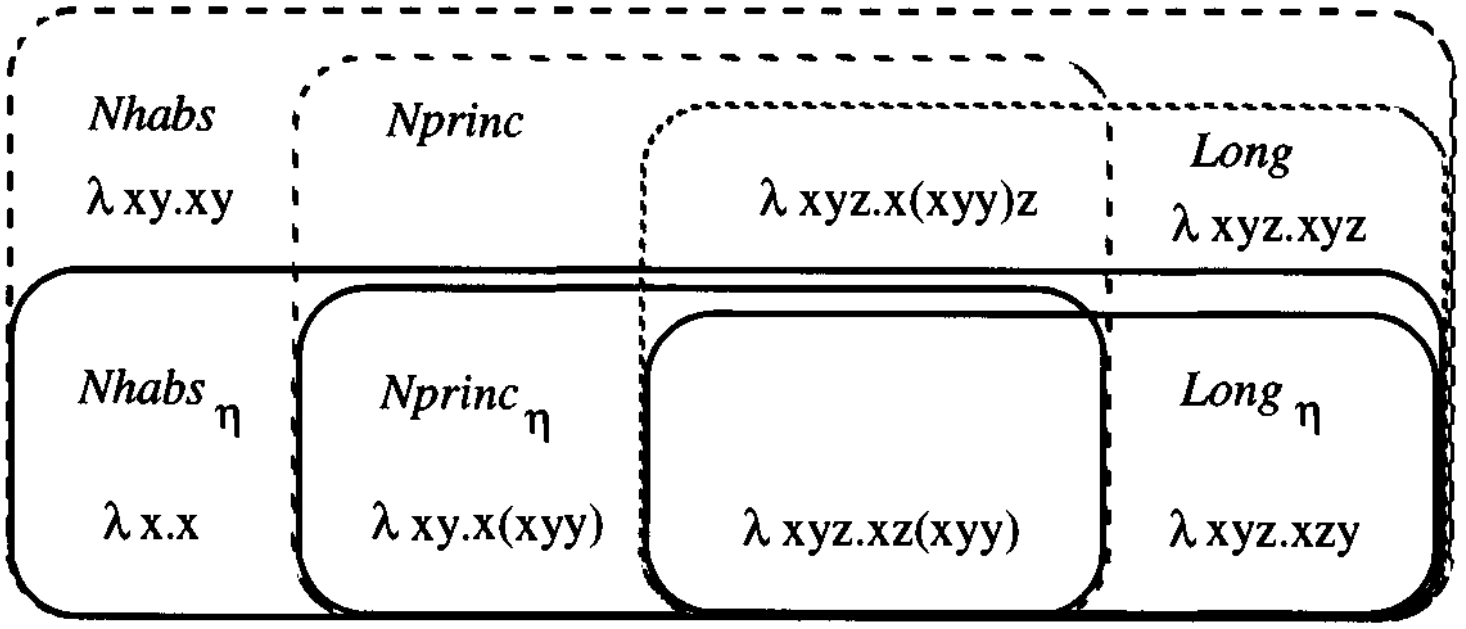
\includegraphics[scale=0.3]{fig2.png}
\end{figure}

\begin{center}
$\tau \equiv (a\to a\to a)\to a \to a \to a$\\[0.5cm]

$
\begin{array}{rlcl}
\mbox{(i)} & \lambda x^{a\to a \to a} \cdot x^{a\to a \to a} & \in & Nhabs_{\eta} - (Nprinc \cup Long)\\ 
\mbox{(ii)} & \lambda x^{a\to a \to a} \, y^{a} \cdot (x\,y)^{a \to a}& \in & Nhabs - Nhabs_{\eta} - (Nprinc \cup Long)\\ 
\mbox{(iii)} & \lambda x^{a\to a \to a} \, y^{a} \, z^{a} \cdot (x\,y\,z)^{a}& \in & Long - Nhabs_{\eta} - Nprinc\\
\mbox{(iv)} & \lambda x^{a\to a \to a} \, y^{a} \cdot (x\,(x\,y\,y))^{a \to a}& \in & Nhabs_{\eta} - Long_{\eta} \\ 
\mbox{(v)} & \lambda x^{a\to a \to a} \, y^{a} \, z^{a} \cdot (x\,(x\,y\,y)\,z)^{a}& \in & Nprinc \cap Long - Nhabs_{\eta} \\ 
\mbox{(vi)} & \lambda x^{a\to a \to a} \, y^{a} \, z^{a} \cdot (x\,z\,(x\,y\,y))^{a}& \in & Nprinc_{\eta} \cap  Long_{\eta}\\ 
\mbox{(vii)} & \lambda x^{a\to a \to a} \, y^{a} \, z^{a} \cdot (x\,z\,y)^{a}& \in &  Long_{\eta} - Nprinc_{\eta}\\ 
\end{array}
$
\end{center}

 
\end{frame}

\begin{frame}
\frametitle{Remarks}
 \begin{itemize}
  \item $Habs(\tau) \neq \emptyset \Longleftrightarrow Nhabs(\tau) \neq \emptyset\,\,\,\,\,$ [\textbf{WN}]
  \item $Habs(\tau) \neq \emptyset \Longleftrightarrow Princ(\tau) \neq \emptyset\,\,\,\,\,\,\,$ [\textbf{converse PT}]
  \item $Habs(\tau) \neq \emptyset \,\,\,{\color{red}\nRightarrow} \,\,\,Nprinc(\tau) \neq \emptyset$
  \item $Princ(\tau) \neq \emptyset \,\,\,{\color{red}\nRightarrow} \,\,\, Nprinc(\tau) \neq \emptyset$
 \end{itemize}

\begin{block}{} 
$\tau$ may have an inhabitant $M$, enven a principal one, such that $PT(M)$ changes when $M$ is reduced to $M*_{\beta}$. 
\end{block}

\begin{exa}[$\tau \equiv a \to a \to a$]
\begin{itemize}
 \item $Nhabs(\tau) = \{\lambda xy \cdot x, \lambda xy \cdot y\}$, but neither of these is principal
 \item But there is a non-normal principal inhabitant: $(\lambda xyz \cdot \mbox{\textbf{K}}(xy)(xz))$\textbf{I}
\end{itemize}


\end{exa}
 
 
\end{frame}




\section{Search strategies}

\begin{frame}
 
 \begin{lem}
   Every type $\tau$ has the form:
   \begin{center}
         $\tau \equiv \tau_1 \rightarrow \cdots \rightarrow \tau_m \rightarrow e$
   \end{center}
  with $m \geq 0$ and $e$ atomic.
\end{lem}
 
\begin{proof}
 \begin{itemize}
  \item if $\tau \equiv a$ then $m = 0$ OK
  \item if $\tau \equiv \sigma \to \rho$ por IH\\
   $\sigma \equiv \sigma_1 \to \cdots \to \sigma_n \to e_{\sigma}$\\
   $\rho \equiv \rho_1 \to \cdots \to \rho_k \to e_{\rho}$\\
   \begin{center}
   $\tau \equiv (\sigma_1 \to \cdots \to \sigma_n \to e_{\sigma}) \to \rho_1 \to \cdots \to \rho_k \to e_{\rho}$
   \end{center}
   
 \end{itemize}
 
\end{proof}
 
\end{frame}


\begin{frame}

\begin{notation}[for $\tau \equiv \tau_1 \rightarrow \cdots \rightarrow \tau_m \rightarrow e$]
\begin{itemize}
 \item The occurrences of $\tau_1,...,\tau_n$ and $e$ will be called \textbf{premises} and \textbf{conclusion} (or \textbf{tail}) of $\tau$\\[0.3cm]
 
 \item $m$ will be called the \textbf{arity} of $\tau$\\[0.3cm]
 
 \item Two type-occurrences will be called \textbf{isomorphic} iff they are occurrences of the same type\\[0.3cm]
 
 \item If the tail-components of $\sigma$ and $\tau$ are isomorphic we may say:
\begin{center}
 $Tail(\sigma) \cong Tail(\tau)$ 
\end{center}
 
\end{itemize}

\end{notation}
  
\begin{mydef}[nf-schemes]
 A nf-scheme is a $\beta$-nf that may contain meta-variables under restrictions:
 \begin{itemize}
  \item[(i)] each nf-scheme is a $\beta$-nf without bound-variables clashes
  \item[(ii)] meta-variables do not bind ($\lambda V$ is forbidden)
  \item[(iii)] in a composite nf-scheme meta-variables only occur in argument positions
  \item[(iv)] each meta-variable in a nf-scheme occurs only once
 \end{itemize}
\end{mydef}
  
\end{frame}


\begin{frame}
\frametitle{Comments}
Let $\tau$ be any type; say $\tau$ has form
\begin{center}
 $\tau \equiv \tau_1 \rightarrow \cdots \rightarrow \tau_m \rightarrow e \,\,\,\,\,\,\, (m \geq 0, e \mbox{ an atom})$
\end{center}
and let $M^{\tau}$ be any $\beta$-nf with type $\tau$. By the lemma \ref{8A5}, $M^{\tau}$ has form
\begin{center}
 $\lambda x_1^{\tau_1} ... \,x_k^{\tau_k} \, . \,
   (v^{(\rho_1 \rightarrow \cdots \rho_n \rightarrow \tau^*)} M^{\rho_1}_1 \cdots
   M^{\rho_n}_n)^{\tau^*})^{(\tau_1 \rightarrow \cdots \tau_k \rightarrow \tau^*)}$
\end{center}
where $0 \leq k \leq m$ and $\tau^* \equiv \tau_{k+1} \to \cdots \to \tau_m \to e$.\\[0.3 cm]
If $M^{\tau} \in Long(\tau)$, then
\begin{itemize}
 \item[(i)] $k = m$ and $\tau^* \equiv e$
 \item[(ii)] the types of $x_1,..,x_m$ coincide with the premises of $\tau$
 \item[(iii)] the tail of the type of $v$ is isomorphic to $Tail(\tau)$
 \item[(iv)] if $M^{\tau}$ is closed then $m \geq 1$ and $v$ is an $x_i \,\,\, (1 \leq i \leq m)$ and
 \begin{center}
  $\tau_i \equiv \rho_1 \to \cdots \to \rho_n \to e$
 \end{center}

\end{itemize}

\end{frame}

\section{Examples of search} 

\begin{frame}
\frametitle{Example $\#(\tau) = 1$}
\begin{block}{ $\tau \equiv (a \to b \to c) \to (a \to b) \to a \to c$}
has exactly one normal inhabitant
\end{block}
\begin{block}{\textbf{S}$^{\tau} \equiv \lambda x^{a \to b \to c}\,y^{a \to b}\,z^a\cdot x\,z\,(y\,z)$}
is its normal inhabitant and is $\in Long(\tau) \cap Princ(\tau)$
\end{block}

\vspace*{0.3 cm}

 \begin{itemize}
  \item[Step 1.] Start by proving that $Long(\tau) = \{\mbox{\textbf{S}}^{\tau}\}$, and looking at the structure of $\tau$; 
  by following the previous comments; we must have:\\[0.2 cm] 
  
			      $\left\{\begin{array}{lcl}
                               m & = & 3 \\
                               e & \equiv & c \\
                               \tau_1 & \equiv & a \to b \to c \\
                               \tau_2 & \equiv & a \to b \\
                               \tau_3 & \equiv & a
                              \end{array}\right.$

 \end{itemize}

 \end{frame}
 
\begin{frame}
\frametitle{Example $\#(\tau) = 1$}
\begin{block}{$M^{\tau} \equiv (\lambda x_1^{\tau_1}\,x_2^{\tau_2}\,x_3^{\tau_3}\cdot(v^{(\rho_1 \to \cdots \rho_n \to c)}\,M_1^{\rho_1}\cdots M_n^{\rho_n})^c)^{(\tau_1 \to \tau_2 \to \tau_3 \to c)} $} 
$\in Long(\tau)$ and has three inital abstracted variables 
\end{block}
\begin{itemize}
 \item By the item (iv) of the previous comments, $v$ must be one of $x_1, x_2, x_3$ whose type's tail is isomorphic to $Tail(\tau) \equiv c$
 \item Then the unique possibly choose is $v \equiv x_1$
 \item $x_1$ must be followed by exactly two arguments, and hence $M$ must have form:
\end{itemize}

\begin{equation}
M \equiv \lambda x_1^{a\to b\to c}\,x_2^{a\to b}\,x_3^a \cdot x_1^{a \to b \to c}\,{\color{red}U^a}\,{\color{blue}V^b}
\end{equation}
\end{frame}

\begin{frame}
\frametitle{Example $\#(\tau) = 1$} 
\begin{itemize}
 \item[Step 2.] Search for suitables ${\color{red}U^a}$ and ${\color{blue}V^b}$\\[0.3cm]
 
 \begin{itemize}
  \item[(i)] by the comments (i), ${\color{red}U^a} \equiv (w\,P_1 \cdots P_r)^a \,\,\,\,\,\,\, (r \geq 0)$
  \item[(ii)]$w$ is an $x_i$ whose type's tail is isomorphic to the tail of the type of ${\color{red}U^a}$
  \item[(iii)] this tail is an occurrence of ${\color{red}a}$, so $w \equiv x_3$
  \item[(iv)] since $x_3$ has no premises so $r = 0$ and \\[0.3cm]
 \end{itemize}
\begin{equation}
 {\color{red}U^a} \equiv x_3^a
\end{equation}
  \begin{itemize}
   \item[(i)] $b$ is an atom then ${\color{blue}V^b}$ cannot be an abstracted
   \item[(ii)] its head must be $x_i$ whose type's tail is an ocurrence of ${\color{blue}b}$
   \item[(iii)] the only possibility is $x_2$
   \item[(iv)] $x_2$ allows only one argument, so \\[0.3cm]
\begin{equation}
 {\color{blue}V^b} \equiv x_2^{a \to b} \, {\color{magenta}W^a}
\end{equation}
  \end{itemize}
\end{itemize}
 
\end{frame}

\begin{frame}
 \frametitle{Example $\#(\tau) = 1$}
\begin{itemize}
 \item[Step 3.] Just as for ${\color{red}U^a}$, the only possibility for ${\color{magenta}W^a}$ is\\[0.3cm]
\begin{equation}
  {\color{magenta}W^a} \equiv x_3^a
\end{equation}
\end{itemize}

\textbf{Conclusion.}

\begin{block}{\begin{center}
               \textbf{S}$^{\tau} \equiv \lambda x_1^{a \to b \to c}\,x_2^{a \to b}\,x_3^a\cdot x_1\,x_3\,(x_2\,x_3)$
              \end{center}}
\begin{center}
there is at most one term (modulo $\equiv_{\alpha}$) in $Long(\tau)$
\end{center}
\end{block}
\begin{itemize}
 \item By the lemma \ref{8A10} and the fact that \textbf{S}$^{\tau}$ is a $\beta\eta$-nf:
 $Nhabs(\tau) = \{S^{\tau}\}$
 \item By the PT algorithm $\tau$ is a principal type of \textbf{S}$^{\tau}$: 
 $Nprinc(\tau) = \{S^{\tau}\}$ 
\end{itemize}

\end{frame}


\begin{frame}
\frametitle{Example $\#(\tau) = m$}
\begin{block}{ $\tau \equiv a \to \cdots \to a \to a\,\,\,\,\,\,\, (m+1 \,a\mbox{'s})$}
for each $m \geq 2$, has exactly $m$ normal inhabitants
\end{block}
\begin{block}{$\Pi^m_i \equiv \lambda x_1^a\,...\,x_m^a\cdot x_i^a\,\,\,\,\,\,\,(1 \leq i \leq m)$}
is its normal inhabitants and is $\in Long(\tau) - Princ(\tau)$. They are called \textbf{projectors} or \textbf{selectors}
\end{block}
 
\end{frame}


\begin{frame}
 \frametitle{Example $\#(\tau) = m$}

\begin{proof}
 \begin{itemize}
  \item By the previous comments, any $M^{\tau} \in Long(\tau)$ must have form\\[0.3 cm]
\begin{center}
 $M^\tau \equiv \lambda x_1^a\,...\, x_m^a \cdot v\,V1 \cdots V_n$
\end{center}
  \item $v \equiv x_i$ for some $i\leq m$
  \item But the types of $x_1, ..., x_m$ have no premises, so $n = 0$. Hence\\[0.3 cm]
\begin{center}
 $M^{\tau} \equiv \lambda x_1^a\,...\,x_m^a \cdot x_i^a$
\end{center}
  \item All selectors are in $Long(\tau)$ and they are $\beta\eta$-nfs. Then by the lemma \ref{8A10}\\[0.3 cm]
\begin{center}
 $Nhabs(\tau) = Long(\tau)$
\end{center}
  \item $m \geq 2$, so by the PT algorithm no selector is in $Nprinc(\tau)$\\[0.3 cm]
\begin{center}
 $Nprinc(\tau) = \emptyset$ 
\end{center}


\end{itemize}
\end{proof}

 
\end{frame}


\begin{frame}
\frametitle{Example $\#(\tau) = 0$}
\begin{itemize}
 \item[(Ex1)] No atomic type has inhabitants
\begin{proof}
 \begin{itemize}
  \item Every type with an inhabitant has a normal one
  \item But every type with a closed normal inhabitant has arity $m \geq 1$  (comments (iv))
 \end{itemize}
\end{proof}
 
 \item[(Ex2)] No type that is skeletal has inhabitants
\begin{proof}
  \begin{itemize}
   \item Let $\tau$ be skeletal and $\tau \equiv \tau_1 \to ... \to \tau_m \to e\,\,\,(m \geq 1)$
   \item If $\tau$ had inhabitants it would have at least one long normal one by the lemma \ref{8A8}
   \item This inhabitant would have form
    $\lambda x_1\,...\,x_m\cdot x_i\,M_1\cdots M_n$
   \item $x_i$ having type $\tau_i$ and the tail of $\tau_i$ being an occurrence of $e$
   \item $\tau$ is skeletal so $e$ cannot occur in any $\tau_i$. Hence $\tau$ has no inhabitants
  \end{itemize}
\end{proof}
\end{itemize}

\end{frame}

\begin{frame}{Example $\#(\tau) = 0$}
\begin{itemize}
  \item[(Ex3)] \textbf{The Peirce's law} ($\tau \equiv ((a \to b) \to a) \to a$) has no inhabitants
 \begin{proof}
  \begin{itemize}
   \item If $M^{\tau} \in Long(\tau)$ then, by the comments, 
   \begin{center}
       $M^{\tau} \equiv \lambda x^{(a\to b) \to a} \cdot v\,U_1\cdots U_n\,\,\,\,\,(n \geq 0)$
   \end{center}
   \item $v \equiv x$, since $M^{\tau}$ is closed. Hence $n = 1$
   \begin{center}By the remarks and the lemma \ref{8A8} 
    \begin{center}\
    $Long(\tau) = \emptyset \Rightarrow Nhabs(\tau) = \emptyset \Rightarrow Habs(\tau) = \emptyset$
    \end{center}
       $M^{\tau} \equiv \lambda x^{(a\to b) \to a} \cdot x^{(a\to b) \to a}\,U^{a\to b}$ 
   \end{center}
    \item Since $a\to b$ has just one premise:
   \begin{center}
    $U^{a\to b} \equiv \lambda y^a \cdot (w\,V_1\cdots V_r)^b\,\,\,\,\, (r \geq 0)$
   \end{center}
    \item $M^{\tau}$ is closed so $w$ must be $x$ or $y$
    \item $w$ must have a type whose tail is an ocurrence of $b$, but neither $x$ nor $y$ has such type
    \item 
  \end{itemize}
 \end{proof}
\end{itemize}
\end{frame}

\begin{frame}
\frametitle{More examples of search}



% $\begin{array}{lcll}
%  P_0  & \equiv & \lambda x \cdot x\,\mbox{\textbf{I}} \\ 
%  P_n  & \equiv & \lambda x \cdot x\,(\lambda y_1 \cdot x\,(\cdots (\lambda y_n \cdot x\,\mbox{\textbf{I}}) \cdots )) &  (n \geq 1), \\
%  Q_{n,i} & \equiv & \lambda x \cdot x\,(\lambda y_1 \cdot x\,(\cdots (\lambda y_n \cdot x\,(\lambda z\cdot y_i)) \cdots )) & (n \geq 1, 1 \leq i \leq n)
%  \end{array}
% $
% \vspace*{0.5cm}
% 
% 



$
 \begin{array}{lllll}\hline\hline
 \mbox{\textbf{Type} } \tau             & Nhabs(\tau)         & Long(\tau)        & Nprinc(\tau)       \\\hline
  a\to a                                 & \mbox{\textbf{I}}   & \mbox{\textbf{I}} & \mbox{\textbf{I}} \\
  a\to b\to a                            & \mbox{\textbf{K}}   & \mbox{\textbf{K}} & \mbox{\textbf{K}} \\
 (a\to b)\to (c \to a) \to c \to b       & \mbox{\textbf{B}}   & \mbox{\textbf{B}} & \mbox{\textbf{B}} \\
 (a\to b\to c)\to b\to a\to c            & \mbox{\textbf{C}}   & \mbox{\textbf{C}} & \mbox{\textbf{C}} \\
 (a\to b\to c)\to (a\to b)\to a\to c     & \mbox{\textbf{S}}   & \mbox{\textbf{S}} & \mbox{\textbf{S}} \\
 (a\to a\to b)\to a\to b                 & \mbox{\textbf{W}}   & \mbox{\textbf{W}} & \mbox{\textbf{W}} \\
 (a\to a) \to a \to a                    & \mbox{\textbf{I}}, \bar{0}, \bar{1}, \bar{2}, ... & \bar{0}, \bar{1}, \bar{2}, ... &\bar{2}, ... \\

  \\\hline\hline
 \end{array}
$

\begin{center}
$
\begin{array}{lcllcl}
 \mbox{\textbf{B}} & \equiv & \lambda x y z \cdot x (y z) & \mbox{\textbf{C}} & \equiv &  \lambda x y z \cdot x z y \\
 \mbox{\textbf{K}} & \equiv & \lambda x y \cdot x &  \mbox{\textbf{I}} & \equiv & \lambda x \cdot x \\
 \mbox{\textbf{S}} & \equiv & \lambda x y z \cdot x z (y z) &  \mbox{\textbf{W}} & \equiv & \lambda x y \cdot x y y \\
 \bar{n} & \equiv & \lambda x y\cdot x^n y
\end{array}
$
\end{center}

\end{frame}

\section{Introduction to the search algorithm}

\begin{frame}{Depth of a term}
\begin{mydef}
 The depth of typed or untyped terms is given by $(m \geq 0)$:
 
 \begin{itemize}
     \item[(i)] $Depth(\lambda x_1\, \cdots \, x_m\, . \, y) = 0$
      \item[(ii)] $Depth(\lambda x_1\, \cdots \, x_m\, . \, y \,M_1 \cdots M_n) = 1+ \underset{1 \leq j \leq n}{Max}\,Depth(M_j)\,\,\,\,\,\,\,$ if $n > 0$
  \end{itemize}
\end{mydef}

\begin{exa}
 \begin{itemize}
  \item $Depth(\lambda u v \cdot u x v x) = Depth(z(\lambda w \cdot y)) = 1$
  \item $Depth(\lambda x \cdot x(z(\lambda w \cdot y))(\lambda u v \cdot u x v x)) = 2$
 \end{itemize}
\end{exa}

\end{frame}

\begin{frame}{Introduction to the search algorithm}
 
 \begin{itemize}
  \item First look for members of $Long(\tau)$ with\\ 
   depth $d = 0$, then $d = 1$, ...\\[0.3 cm]
  \item The output is the sequence  of finite sets $\mathcal{A}(\tau,0),\,\mathcal{A}(\tau,1),\,\mathcal{A}(\tau,2),\,...$ as aproximations of $Long(\tau)$\\[0.3 cm]
  \item Those in $\mathcal{A}(\tau,d)$ will look like typed $\beta$-nf's with depth $\leq d$ but with some 'holes' (meta-variables)\\[0.3 cm]
  \item To construct $\mathcal{A}(\tau,d+1)$ the aproximations in $\mathcal{A}(\tau,d)$ will be extended by replacing their meta-variables with nf-schemes with depth 1
 \end{itemize}

 
\end{frame}

\begin{frame}{The search algorithm}
          It is an algorithm to find Long terms to an type, but with a
          limitaded depth.
          $\mathcal{A}(\tau,0)$

          \begin{itemize}
                 \item[(i)] If $\tau$ is atomic, outputs empty set

                 \item[(ii)] Otherwise, outputs $\{V^{\tau}\}$, where
                   $V$ is a meta-variable
          \end{itemize}
     
\end{frame}

\begin{frame}
          Assume the output of $\mathcal{A}(\tau,d)$ is ready to
          compute $\mathcal{A}(\tau,d+1)$.

          \begin{itemize}
                 \item[(i)] If the output is the empty set or it not
                   contains any meta-variable in any term,
                   stop. $\mathcal{A}(\tau,d+1)$ is undefined and the
                   algorithm just outputs the sequence
                   $(\mathcal{A}(\tau,0), \cdots, \mathcal{A}(\tau,d))$
          \end{itemize}
\end{frame}

\begin{frame}
      \begin{mydef}
            A proper nf-schemes is one that contain some meta-variable
      \end{mydef}

      For each meta-variable $V^{\rho}$ in each proper nf-scheme $X^{\tau}$ in
      $\mathcal{A}(\tau,d))$
      Consider $\rho$ as

      \begin{center}
            $\rho \equiv \sigma_1 \to \cdots \to \sigma_m \to a$
      \end{center}

      List each $\sigma_i$ such that $tail(\sigma_i) \cong a$. For all
      that, define:
      \begin{center}
            $\sigma_i \equiv \sigma_{i,1} \to \cdots \to \sigma_{i,n_i}
            \to a$
      \end{center}

      and
      
      \begin{center}
             $Y^{\rho}_i \equiv \lambda x^{\sigma_1}_1 \cdots
             x^{\sigma_m}_m \cdot (x^{\sigma_i}_i
             V^{\sigma_{i,1}}_{i,1} \cdots V^{\sigma_{i,n_i}}_{i,n_i})^a$
      \end{center}

      where x`s and V`s are new variables and
      meta-variables. $Y^{\rho}$ is called a suitable replacement of $V^{\rho}$.
\end{frame}

\begin{frame}
     List the abstractors tha cover $V^{\rho}$ in orther that they
     occur in $X^{\tau}$ :

     \begin{center}
          $\lambda z^{\zeta_1}_1, \cdots, \lambda z^{\zeta_t}_t$
     \end{center}

     For each $\zeta_j$ such that $tail(\zeta_j) \cong a$ has the
     form:

     \begin{center}
           $\zeta_j \equiv \zeta_{j,1} \to \cdots \to \zeta_{j,h_j}
           \to a$
     \end{center}

     Define:
     \begin{center}
            $Z^{\rho}_j \equiv \lambda x^{\sigma_1}_1 \cdots x^{\sigma_m}_m
     \cdot (z^{\zeta_j}_j V^{\zeta_{j,1}}_{j,1} \cdots
     V^{\zeta_{j,h_j}}_{j,h_j})^a $
     \end{center}

     where x`s and V`s are new variables and
     meta-variables. $Z^{\rho}_j$ is a suitable substitution of $V^{\rho}$
\end{frame}

\begin{frame}
     Each $X^{\tau}$ in $\mathcal{A}(\tau,d)$ generates some lists of suitable
     substitution for all meta-variable in $X^{\tau}$. But if
     $X^{\tau}$ does not have this kind of list, discart it.

     $\mathcal{A}(\tau,d+1)$ is each substitution of meta-variables
     $X^{\tau}$ by there suitable substitution in a list of suitable replacement.
\end{frame}

\begin{frame}{Example}
  \begin{exa}
      $\tau = a \to b \to c$

      $\mathcal{A}(\tau,0) = \{V^{\tau}\}$

      $\mathcal{A}(\tau,1) = \emptyset$
  \end{exa}
\end{frame}

\begin{frame}{Search algorithms properties}
	\begin{lem}
     \begin{enumerate}
           \item Each member of $\mathcal{A}(\tau,d)$ is a closed long
             term typed $\tau$ and is either:
             \begin{itemize}
                     \item a proper nf-scheme with depth d or
                     \item a term with depth d-1
              \end{itemize}
              \item $\mathcal{A}(\tau,d)$ is finite
               \item $Long(\tau,d) \subseteq \mathcal{A}(\tau,0) \cup \cdots
                 \cup\mathcal{A}(\tau,d+1)$
                 \item $Long(\tau) = \bigcup_{d \geq 0} \mathcal{A}_{terms}(\tau,d)$
      \end{enumerate}
      \end{lem}

      \begin{proof}
             \begin{itemize}
                      \item Item 1 and 2 is made by induction in $d$
                      \item Item 3 is kind of that but with new
                        definitions.
                       \item 4 is a corolary
             \end{itemize}
      \end{proof}
      
\end{frame}

\begin{frame}
  \begin{mydef}
        $\mathbb{D}(\tau) = |\tau| \times ||\tau||$

        Where $|\tau|$ is the number of atom occurences and $||\tau||$
        is the number of distinct atom in $\tau$.
  \end{mydef}

  \begin{lem}[Stretching lemma]
      If $Long(\tau)$ has a member $M^{\tau}$ with depth bigger
      than $||\tau||$, so given any integer, there is another one
      bigger than this integer.
   \end{lem}

   \begin{lem}[Shirinking lemma]
            If $Long(\tau)$ has a member $M^{\tau}$ with depth bigger
            than $\mathbb{D}(\tau)$ there is a member $N^{\tau}$

            Such that

            $\mathbb{\tau}-||\tau|| \leq Depth(N^{\tau}) \leq \mathbb{D}(\tau)$
    \end{lem}

\end{frame}


% \section{First conclusions}
% 
% \begin{frame}{First conclusions}
% \begin{itemize}
%  \item The point is searching for \textbf{long normal forms}\\[0.5cm]
%  
%  \item The the \textbf{Search} and the \textbf{Count Algorithms} will work with the idea of \textbf{nf-schemes} and analisis in the term's \textbf{depth}\\[0.5cm]
%  
%  \item Intuitionist implicational logic is consistent in the sense that not all formulae are provable
% \end{itemize}
% \end{frame}
% 



% \section{The search algorithm}
% 
% \begin{frame}
% 
% 
% 
%  
% \end{frame}
% 
% \section{The Counting algorithm}
% 
% \begin{frame}
% 
% 
% 
%  
% \end{frame}
% 

% here the slides for section 8E
% in this file, the slides for section 8E
\section{8E - The Structure of a nf-scheme}

\subsection{Overview and Motivation}
% overview
\begin{frame}{8E - The Structure of a nf-scheme}
    This section is about analysing the structure of an arbitrary long typed nf-scheme. 
\end{frame}

% motivation
\begin{frame}{Motivation}
    Earlier sections left the stretching and shrinking lemmas unproved (8D2 and 8D3), 
    as well as the completeness part of the searching theorem for \texttt{Long}($\tau$) (8C5(iii)). 
    
    \medskip
    
    \begin{itemize}
        \item \textbf{8E} - We lay the foundation by analysing the structure of an arbitrary long
        typed nf-scheme. 
        \item \textbf{8F} - Having the necessary foundation, we fill the mentioned gaps. 
    \end{itemize}
\end{frame}

\subsection{Key Role, Remarks and Notations}
\begin{frame}{Structured Proofs à la Leslie Lamport}
    In this presentation, the mathematical proofs are presented as structured proofs à la Leslie Lamport \cite{lamport1, lamport2}.
\end{frame}

\begin{frame}{Notation for Components}
We will underline a term $Y$ when we want to indicate that it is being analysed as a component of a term $X$.
\end{frame}

\begin{frame}{Organization of the Present Section}
The early parts of this section will apply to both typed and untyped nf-schemes. Therefore, when we write nf-schemes, types will be omitted. 

\medskip

The final parts of this section will only apply to typed nf-schemes, so types will be displayed. 
\end{frame}

\begin{frame}{Key Role}
    A key role in our analysis will be played by a slightly strengthened form of the subformula property. This property says that the types of all the components of a closed $\beta$-nf $M^\tau$ are subtypes of $\tau$. 
    
    \medskip 
    
    This way, as the algorithm searches deeper and deeper, the types of the components we are working with remain drawn from the same fixed finite set. 
\end{frame}


% TODO: if i want put a slide here about notation of positions.

\begin{frame}{nf-scheme}
\begin{remark}
     A nf-scheme is essentially a $\beta$-nf that may contain meta-variables under suitable restrictions. 
\end{remark}
\end{frame}

\begin{frame}{nf-scheme}
\begin{remark}
According to 8A5, every non-atomic nf-scheme $X$ can be expressed uniquely in the form: 
\begin{equation*}
    X \equiv \lambda x_1 \ldots x_m.v Y_1 \ldots Y_n
\end{equation*}
with $m+n \geq 1$ and where $v$ is one of the $x_i$ if $X$ is closed. 

\medskip

The head and arguments of $X$ are $v$ and $Y_1, \ldots, Y_n$. If $X$ is an atom its head is $X$ and it has no arguments. 

\medskip 

The construction-tree of such an X is shown in Fig \ref{fig_construction}. Note that the position of $Y_i$ is: $0^{m} 1^{n-i} 2$, for $1 \le i \le n$. 
\end{remark}
\end{frame}

\begin{frame}{An Example of a Construction Tree}
\begin{figure}
    \centering
    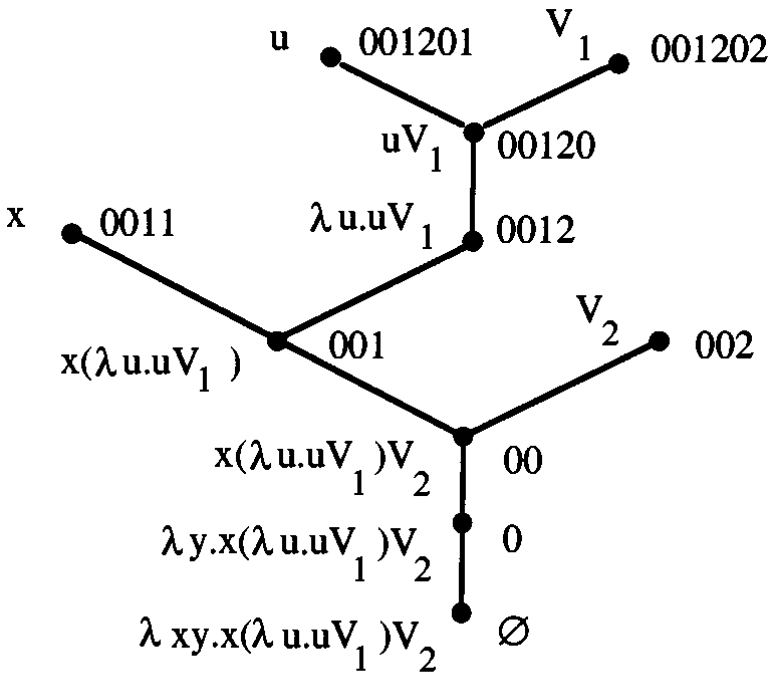
\includegraphics[width=7cm]{fig4.png}
    \caption{Construction Tree for $\lambda xy.x(\lambda u.uV_1)V_2$.
    Figure obtained from \cite{hindley}.}
    \label{fig_construction}
\end{figure}
    
\end{frame}

\subsection{The Foundation for 8F}
\begin{frame}{Subarguments}
\begin{definition}[8E2 in Hindley's]
A subargument of a typed or untyped nf-scheme $X$ is a component that is an argument of $X$ or an argument of a proper component of $X$.
\end{definition}
\end{frame}

\begin{frame}{Lemma 8E2.1}
\begin{lemma}[8E2.1 in Hindley's]
A component \underbar{$Y$} of a typed or untyped nf-scheme $X$ is a subargument iff 
its position is not $\emptyset$ and the last symbol in its position is 2. 
\end{lemma}

\begin{proof}
\pfsketch \ 
By induction on $|X|$. One can, for instance, consider the subarguments in the tree of Figure \ref{fig_construction}.
\end{proof}
\end{frame}

\begin{frame}{Remarks about Subarguments}
\begin{remark}[8E2.2(i) in Hindley's]
All occurrences of meta-variables in a composite nf-scheme are subarguments.
\begin{proof}
\pf \ By restriction 8C1(iii) in the definition of nf-scheme. 
\end{proof}
\end{remark}

\medskip

\begin{remark}[8E2.2(ii) in Hindley's]
A subargument of a subargument of $X$ is a subargument of $X$.
\begin{proof}
\pf \ By the definition of subargument. 
\end{proof}
\end{remark}
\end{frame}

\begin{frame} {2-length and depth}
\begin{mydef}[8E3 in Hindley's]
The 2-length of a position string $p$ is the number of 2's in $p$. 
\end{mydef} 

\medskip 
\begin{mydef}[8E3 in Hindley's]
The depth in $X$ of a subargument $\underbar{Z}$ of $X$ is the 2-lenght of its position. 
\end{mydef}

\begin{remark}[8E3 in Hindley's]
The depth in $X$ of a subargument $\underbar{Z}$ is the number of right-hand choices made when ``travelling up'' the tree of $X$ from the bottom node to $\underbar{Z}$.  
\end{remark}
\end{frame}

\begin{frame}{Lemma 8E3.1}

\begin{lemma}[8E3.1 in Hindley's]
Let $X$ be a typed or untyped nf-scheme with $Depth(X) \geq 1$, where the $Depth$ of an nf-scheme is defined as in 8A6. Then: 
\begin{enumerate}
\item $Depth(X)$ is the maximum of the depths in $X$ of all subarguments in $X$, 
\item $X$ has at least one subargument whose depth in $X$ is the same as $Depth(X)$, and each such subargument is an atom or abstracted atom. 
\end{enumerate} 
\end{lemma}

\begin{proof}
\pfsketch \ By induction on $|X|$, using 8A6. 
\end{proof} 
\end{frame} 

\begin{frame}{Argument-Branch}
\begin{mydef}[8E4 in Hindley's]
If $Z$ is a subargument of a typed or untyped nf-scheme $X$, the \textbf{argument-branch} from $X$ to $Z$ is the sequence: 

\begin{equation*}
\langle \underbar{Z}_0, \underbar{Z}_1, \ldots, \underbar{Z}_k  \rangle
\end{equation*}

such that $\underbar{Z}_0 \equiv \underbar{X}$, $\underbar{Z}_k \equiv \underbar{Z}$ and for each $i = 1, \ldots, k$, we have   $\underbar{Z}_i$ is an argument of $\underbar{Z}_{i-1}$.

\medskip

It is \textbf{unextendable} iff $\underbar{$Z$}$ is an atom or abstracted atom. 

\medskip 

Its \textbf{length} is $k$ (not $k+1$). 
\end{mydef}
    
\end{frame}

\begin{frame}{Lemma 8E4.1}
\begin{lemma}[8E4.1 in Hindley's]
For any typed or untyped nf-scheme $X$:
\begin{enumerate}
\item The depth in $X$ of a subargument $\underbar{$Z$}$ is the same as the length of the argument-branch from $\underbar{X}$ to $\underbar{Z}$, 
\item $Depth(X)$ is the maximum of the lengths of all argument-branches in $X$. 
\end{enumerate}
\end{lemma}

\begin{proof}
\pfsketch \ For (1) use induction on $|X|$, for (2) use 8E3.1.  
\end{proof}
\end{frame}

\begin{frame}{IA, CA}
\begin{mydef}[8E5 in Hindley's]
Let $\underbar{$Z$}$ be a subargument of a typed or untyped nf-scheme $X$, for instance: 

\begin{equation*} 
Z \equiv \lambda x_1 \ldots x_m.y Z_1 \ldots Z_n \tag{$m \ge 0, n \ge 0$}
\end{equation*}

The \textbf{Initial Abstractors sequence IA(Z)} is the (possibly empty) sequence: 
\begin{equation*}
    IA(Z) = \langle x_1, \ldots, x_m \rangle
\end{equation*}

The \textbf{Covering Abstractors sequence CA(\underline{Z}, X)} is defined as: 
\begin{equation*}
    CA(\underbar{Z}, X) = \langle z_1, \ldots, z_q \rangle, 
\end{equation*}

where $\underline{\lambda z}_1$, \ldots, $\underline{\lambda z}_q$ are the abstractors in $X$ whose scopes contain \underbar{$Z$}, written in the order they occur in $X$ from left to right. Also, define: 
\begin{align*}
    Length(IA(Z)) &= m, \\
    Length(CA(\underbar{Z}, X)) &= q.
\end{align*}

\end{mydef}
\end{frame} 

\begin{frame}{IA, CA}
\begin{remark}[8E5.1 in Hindley's]
\begin{enumerate}
    \item If $X$ has no bound-variable clashes, the members of $IA(Z)$ are distinct and so are those of $CA(\underbar{Z}, X)$. 
    \item $IA(Z)$ and $CA(\underbar{Z}, X)$ are sequences of variables, not components. 
    \item For typed nf-schemes each variable in $IA(Z)$ or $CA(\underbar{Z}, X)$ is typed. 
    \item If the argument-branch from \underbar{$X$} to \underbar{$Z$} is $\langle \underbar{Z}_0, \ldots, \underbar{Z}_k \rangle$ ($k \geq 1)$, then: 
    \begin{equation*}
        CA(\underbar{Z}, X) = IA(Z_0) * \ldots * IA(Z_{k-1})
    \end{equation*}
    where ``*'' denotes concatenation of sequences.
\end{enumerate}
\end{remark} 
\end{frame}

\begin{frame}{Warning}
The remaining part of this section applies only for typed nf-schemes. 
\end{frame}

\begin{frame}{IAT}
\begin{mydef}[IAT]
Let \underbar{$Z^\sigma$} be a subargument of a typed nf-scheme $X^\tau$, say: 
\begin{equation*}
    Z^{\sigma} \equiv \lambda x_{1}^{\sigma_1}
    \ldots x_{m}^{\sigma_m}.y Z_1 \ldots Z_n     \tag{$m \geq 0, n \geq 0$}
\end{equation*}

The \textbf{Initial Abstractors' Types Sequence ($IAT(Z^\sigma)$)} is defined as: 
\begin{equation*}
    IAT(Z^{\sigma}) = \langle \sigma_1, \ldots, \sigma_m \rangle; 
\end{equation*}

And we also define:
\begin{equation*}
    Length(IAT(Z^\sigma)) = m
\end{equation*} 
\end{mydef}
\end{frame}

\begin{frame}{Premises}
    If $\rho \equiv \rho_1 \rightarrow \ldots \rightarrow \rho_m \rightarrow a$, we call $\rho_1, \ldots, \rho_m$ the premises of $\rho$ and we call $a$ the tail of $\rho$.
\end{frame}

\begin{frame}{Positions in a Term}
Consider $\tau \equiv (a \rightarrow b \rightarrow c) \rightarrow (a \rightarrow b) \rightarrow a \rightarrow c$. 
\begin{figure}
    \centering
    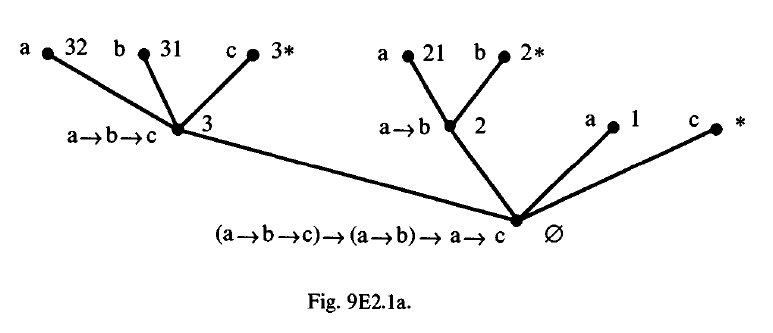
\includegraphics[width=7cm]{subpremise.png}
    \caption{Positions in the term $\tau \equiv (a \rightarrow b \rightarrow c) \rightarrow (a \rightarrow b) \rightarrow a \rightarrow c$.
    Figure obtained from \cite{hindley}.}
    \label{subpremise1}
\end{figure}
\end{frame}

\begin{frame}{Subpremises}
    A subpremise of $\tau$ is a premise of some component of $\tau$ (possibly of $\tau$ itself).
\end{frame}

\begin{frame}{Subpremises}
    \begin{exa}
    \label{ex_subpremises}
    Let $\tau \equiv (a \rightarrow b \rightarrow c) \rightarrow (a \rightarrow b) \rightarrow a \rightarrow c$ (see Figure \ref{subpremise1}). Let's represent subpremisses as triples ``$\langle \text{term}, \text{position}, \tau  \rangle$''. The six subpremisses of $\tau$ are: 
    \begin{enumerate}
        \item $\langle a, 1, \tau \rangle$,
        \item $\langle a \rightarrow b, 2, \tau \rangle$,
        \item $\langle a \rightarrow b \rightarrow c, 3, \tau \rangle$, 
        \item $\langle a, 21, \tau \rangle$,
        \item $\langle b, 31, \tau \rangle$,
        \item $\langle a, 32, \tau \rangle$. 
    \end{enumerate}
    \end{exa}
\end{frame}

\begin{frame}{Positive Subpremises}
    A subpremise of $\tau$ is positive if and only if its position has even length (the symbol $*$ does not count when computing the length). 
    
    \medskip 
    
    In Example \ref{ex_subpremises} the positive subpremises are: 
    \begin{enumerate}
        \item $\langle a, 21, \tau \rangle$,
        \item $\langle b, 31, \tau \rangle$,
        \item $\langle a, 32, \tau \rangle$.
    \end{enumerate}
    
\end{frame}

\begin{frame}{NSS}
\begin{mydef}
$NSS(\tau)$ is the set of all finite sequences 
$\langle \sigma_1, \ldots, \sigma_n \rangle \ \ (n \geq 1)$ such that: 
\begin{equation}
    \sigma_1 \rightarrow \ldots \rightarrow \sigma_n \rightarrow a
\end{equation} 
is positive in $\tau$. 
\end{mydef}

\begin{remark}
Each member of $NSS(\tau)$ is called a negative subpremise-sequence, because it is a sequence of terms that have occurrences as negative subpremises in $\tau$.  
\end{remark}
\end{frame}

\begin{frame}{NSS}
\begin{exa}
\label{ex_nss}
Let $\tau \equiv (a \rightarrow (b \rightarrow d \rightarrow c) \rightarrow d)\rightarrow (a \rightarrow b \rightarrow c) \rightarrow d \rightarrow d$. 

We have $NSS(\tau) = \{ \langle a \rightarrow (b \rightarrow d \rightarrow c) \rightarrow d, a \rightarrow b \rightarrow c, d \rangle, \langle b, d \rangle \}$.
\end{exa}
\end{frame}

\begin{frame}{NSS}
\begin{proof}
\pf
\step{1}{$NSS(\tau) \supseteq \{ \langle a \rightarrow (b \rightarrow d \rightarrow c) \rightarrow d, a \rightarrow b \rightarrow c, d \rangle, \langle b, d \rangle \}$}
\begin{proof}

\step{1-1}{$\langle a \rightarrow (b \rightarrow d \rightarrow c) \rightarrow d, a \rightarrow b \rightarrow c, d \rangle \in NSS(\tau)$}
\begin{proof}
By definition, since:
\begin{equation*}
(a \rightarrow (b \rightarrow d \rightarrow c) \rightarrow d)\rightarrow (a \rightarrow b \rightarrow c) \rightarrow d \rightarrow d
\end{equation*}
is positive in $\tau$, as it has position $\emptyset$, of even length. 
\end{proof}

\medskip 

\step{1-2}{$\langle b, d \rangle \in NSS(\tau)$}
\begin{proof} 
By definition, since: 
\begin{equation*}
    b \rightarrow d \rightarrow c
\end{equation*}
is positive in $\tau$ as it has position 31, of even length. 
\end{proof} 

\end{proof}

\medskip

\step{2}{$NSS(\tau) \subseteq \{ \langle a \rightarrow (b \rightarrow d \rightarrow c) \rightarrow d, a \rightarrow b \rightarrow c, d \rangle, \langle b, d \rangle \}$}
\begin{proof} 
By checking that no other finite sequence $\langle \sigma_1, \ldots, \sigma_n \rangle$ is such that $\sigma_1 \rightarrow \ldots \rightarrow \sigma_n \rightarrow a$ is positive in $\tau$.  
\end{proof}
\end{proof}
\end{frame}

\begin{frame}{NSS}
\begin{mydef}
The set of all the members of the sequences in $NSS(\tau)$ will be called $\cup NSS(\tau)$
\end{mydef}

\begin{exa}
In Example \ref{ex_nss}, we had: 
\begin{equation*}
    NSS(\tau) = \{ \langle a \rightarrow (b \rightarrow d \rightarrow c) \rightarrow d, a \rightarrow b \rightarrow c, d \rangle, \langle b, d \rangle \}
\end{equation*}
Therefore,
\begin{equation*}
    \cup NSS(\tau) = \{ a \rightarrow (b \rightarrow d \rightarrow c) \rightarrow d, a \rightarrow b \rightarrow c, d, b \}
\end{equation*}

\end{exa}

\end{frame}

\begin{frame}{Lemma 8E7}
\begin{lemma}[8E7 in Hindley's]
If \underbar{$Z^\sigma$} is a subargument of a closed long typed nf-scheme $X^\tau$, then 
\begin{enumerate}
    \item $\sigma$ occurs as a positive subpremise in $\tau$ (as defined in 9E6-8), 
    \item If $\sigma$ is an atom, $IAT(Z^\sigma) = \emptyset$, 
    \item If $\sigma$ is composite, $IAT(Z^\sigma) \in NSS(\tau)$ (defined in 9E9),
    \item $NSS(\sigma) \subseteq NSS(\tau)$.
\end{enumerate}
\end{lemma}
\end{frame}

\begin{frame}[allowframebreaks]{Proof of Lemma 8E7}
\begin{proof} 
\pf
\step{1}{$\sigma$ occurs as a positive subpremise in $\tau$ (as defined in 9E6-8).}
% TODO: comment that in this proof, you can't do induction if you start with an empty context. 
\begin{proof} 
\medskip 
\step{1-1}{If $X^\tau$ is a long member of $\mathbb{TNS}$($\Gamma$) and $\Gamma = \{u_1: \theta_1, \ldots, u_p: \theta_p, V_1: \phi_1, \ldots, V_q: \phi_q\}$ and \underbar{$Z^\sigma$} is a subargument of $X^\tau$, then $\sigma$ occurs as a positive subpremise of $\theta_1 \rightarrow \ldots \rightarrow \theta_p \rightarrow \tau$.}
\begin{proof}
The proof is by induction on $|X^\tau|$.

\medskip 

\step{1-1-1}{\textbf{Basis} If $X^\tau$ is an atom there is no \underbar{$Z^\sigma$} subargument of $X^\tau$, and the conclusion holds vacuously.}

\framebreak

\step{1-1-2}{\textbf{Induction Step}}
\begin{proof}
\step{1-1-2-1}{X has the form: 
\begin{equation*}
    (\lambda x_{1}^{\tau_1} \ldots x_{m}^{\tau_m}.
    (y^{(\rho_1 \rightarrow \ldots \rightarrow \rho_n \rightarrow e)}
    X_{1}^{\rho_{1}} \ldots X_{n}^{\rho_{n}} )^{e}
    )^{\tau_1 \rightarrow \ldots \rightarrow \tau_m \rightarrow e}
\end{equation*} 
where $m, n \geq 0$ and $\tau \equiv \tau_1 \rightarrow \ldots \rightarrow \tau_m \rightarrow e$.}

\medskip 

\step{1-1-2-2}{\casePfkwd \ $Z^{\sigma} \equiv X_{j}^{\rho_j}$.}
\begin{proof} 
\noindent

\step{1-1-2-2-1}{Since $Z^{\sigma} \equiv X_{j}^{\rho_j}$, we have $\sigma \equiv \rho_j$.}

\step{1-1-2-2-2}{Each of $\rho_1, \ldots, \rho_n$ occurs as a positive subpremise of $\theta_1 \rightarrow \ldots \rightarrow \theta_p \rightarrow \tau$.}
\begin{proof}
\noindent
\step{1-1-2-2-2-1}{Using the notation of  \stepref{1-1-2-1} and \stepref{1-1}, we have that either $y \equiv x_i$ for some $i \le m$ or $y \equiv u_i$ for some $i \le p$.}
\step{1-1-2-2-2-2}{\casePfkwd \ $y \equiv x_i$. We have that $\rho_1 \rightarrow \ldots \rightarrow \rho_n \rightarrow e \equiv \tau_i$. Then, the position of each $\rho_j$ in $\theta_1 \rightarrow \ldots \rightarrow \theta_p \rightarrow \tau$ has length 2, making it a positive subpremise.}
\step{1-1-2-2-2-3}{\casePfkwd \ $y \equiv u_i$. Then $\rho_1 \rightarrow \ldots \rightarrow \rho_n \rightarrow e \equiv \theta_i$. Then, the position of each $\rho_j$ has length 2, making it a positive subpremise.}
\end{proof}

\end{proof} 

\medskip 

\step{1-1-2-3}{\casePfkwd \ $Z^{\sigma}$ is a subargument of $X_{j}^{\rho_j}$.}

\begin{proof}
\noindent
\step{1-1-2-3-1}{$X_{j}^{\rho_j}$ is a long member of $\mathbb{TNS}(\{x_{1}:\tau_1, \ldots, x_{m}:\tau_{m} \} \cup \Gamma)$}
\step{1-1-2-3-2}{By IH, $\sigma$ occurs as a positive subpremise of
\begin{equation*}
    \tau_1 \rightarrow \ldots \rightarrow \tau_m \rightarrow \theta_1 \rightarrow \ldots \rightarrow \theta_p \rightarrow \rho_j
\end{equation*}.}
\step{1-1-2-3-3}{\casePfkwd \ $\sigma$ is a positive subpremise of $\rho_j$. Then, by using the result $\langle 5 \rangle 2$ of branch $\langle 4 \rangle 2$ (notice the result holds because we can repeat the argument),  we conclude.}
\step{1-1-2-3-4}{\casePfkwd \ $\sigma$ is a negative subpremise of one of $\tau_1, \ldots, \tau_m, \theta_1, \ldots, \theta_p$. Then $\sigma$ will be a positive subpremise of $\theta_1 \rightarrow \ldots \rightarrow \theta_p \rightarrow \tau$.}
\end{proof}

\end{proof}

\end{proof}

\framebreak

\step{2-2}{Since $X^\tau$ is closed, we can apply \stepref{1-1} with $\Gamma = \emptyset$ and conclude.}

\end{proof}

\framebreak

\step{2}{If $\sigma$ is an atom, $IAT(Z^\sigma) = \emptyset$.}
\begin{proof}
\step{2-1}{$IAT(Z^\sigma)$ coincides with the sequences of all premises of $\sigma$.}
\begin{proof}
\step{2-1-1}{$Z^\sigma$ is long.}
\step{2-1-2}{\letPfkwd \  $IAT(Z^\sigma) = \langle \sigma_1, \ldots, \sigma_m \rangle$. Since $Z^\sigma$ is long, $\sigma \equiv \sigma_1 \rightarrow \ldots \rightarrow \sigma_m \rightarrow e$.}
\end{proof}
\step{2-2}{Since $\sigma$ is an atom, there are no premises. By \stepref{2-1}, $IAT(Z^\sigma) = \emptyset$.}
\end{proof}

\framebreak

\step{3}{If $\sigma$ is composite, $IAT(Z^\sigma) \in NSS(\tau)$ (defined in 9E9)}
\begin{proof}
\step{3-1}{$IAT(Z^\sigma) \in NSS(\sigma)$.}
\begin{proof}
\step{3-1-1}{$Z^\sigma$ is long.}
\step{3-1-1}{\letPfkwd \ $IAT(Z^\sigma) = \langle \sigma_1, \ldots, \sigma_m \rangle$. Then, since $Z^\sigma$ is long, $\sigma \equiv \sigma_1 \rightarrow \ldots \rightarrow \sigma_m \rightarrow e$.}
\step{3-1-3}{By \stepref{3-1-1}, and the definition of $NSS(\sigma)$ (which is only defined for $\sigma$ composite) we conclude.}
\end{proof}
\step{3-2}{$NSS(\sigma) \subseteq NSS(\tau)$.}
\begin{proof}
It will be proved in $\langle 1 \rangle$4.
\end{proof}
\end{proof}

\framebreak

\step{4}{$NSS(\sigma) \subseteq NSS(\tau)$.}
\begin{proof}
\step{4-1}{By \stepref{1}, $\sigma$ occurs as a positive subpremise in $\tau$.} 
\step{4-2}{By the technical lemma 9E9.2(iii), since $\sigma$ occurs as a positive subpremise of $\tau$, we have $NSS(\sigma) \subseteq NSS(\tau)$.}
\end{proof}
\end{proof}
\end{frame}

\begin{frame}{Lemma 8E7}
\begin{remark}
Notice that Lemma 8E7 connects $IAT(Z^\sigma)$, which in general depends on the structure of $Z^\sigma$ and hence implicitly on that of $X^\tau$, with $NSS(\tau)$, which depends on $\tau$ and nothing else. 
\end{remark}
\end{frame}


\begin{frame}{Corollary 8E7.1}
\begin{corollary}[8E7.1 in Hindley's]
    If $X^\tau$ is a closed long typed nf-scheme, the type of each meta-variable in $X^\tau$ either occurs as a positive subpremise of $\tau$ or is $\tau$ itself. 
\end{corollary}

\begin{proof}
\step{1}{\casePfkwd \ $X^\tau$ is a composite nf-scheme.}
\begin{proof}
\step{1-1}{\letPfkwd \ $Z^\sigma$ be an arbitrary metavariable in $X^\tau$.}
\step{2-1}{An occurrence of $Z^\sigma$ in $X^\tau$ is a subargument.}
\step{3-1}{Then, by Lemma 8E7, $\sigma$ occurs as a positive subpremise of $\tau$.}
\end{proof}

\medskip 

\step{2}{\casePfkwd \ $X^\tau$ is an atomic nf-scheme.}
\begin{proof}
In this case, $X^\tau$ is a meta-variable. 
\end{proof} 
\end{proof}

\end{frame}

\begin{frame}[allowframebreaks]{Corollary 8E7.2}
\begin{corollary}[8E7.2 in Hindley's]
If $X^\tau$ is a closed long typed nf-scheme and \underbar{$Z^\sigma$} is a subargument of $X^\tau$ or \underbar{$Z^\sigma$} $\equiv$ \underbar{$X^\tau$}, then: 
\begin{enumerate}
    \item Length($IA(Z^\sigma)$) = Length($IAT(Z^\sigma)$) $\leq |\tau| - 1$, 
    \item Length($CA($\underbar{$Z^{\sigma}$}, $X^\tau$)) $\le (|\tau|-1) \times$ Depth($X^\tau$), 
    \item If $\underline{\lambda v}_{1}^{\rho_1}$, $\ldots$, $\underline{\lambda v}_{r}^{\rho_r}$ are all abstractors in $X^\tau$ (not just the initial ones), then $\{\rho_1, \ldots, \rho_r \}$ has $\le |\tau|-1$ distinct members.  
\end{enumerate}
\end{corollary}
\end{frame}

\begin{frame}[allowframebreaks]{Corollary 8E7.2}
\begin{proof}
\step{1}{Length($IA(Z^\sigma)$) = Length($IAT(Z^\sigma)$) $\leq |\tau| - 1$}

\begin{proof}

\medskip 

\step{1-1}{\letPfkwd \  $Z^\sigma \equiv \lambda x_{1}^{\sigma_1} \ldots x_{m}^{\sigma_m}.
y Z_{1}\ldots Z_{n}$}

\medskip 

\step{1-2}{Length($IA(Z^\sigma)$) = Length($IAT(Z^\sigma)$) $= m$.}
\begin{proof}
By definition, $IA(Z^\sigma) = \langle x_1, \ldots, x_m \rangle$ and $IAT(Z^\sigma) = \langle \sigma_1, \ldots \sigma_m \rangle$. 
\end{proof}

\medskip 

\step{1-3}{Length($IAT(Z^\sigma)$) $\leq |\tau| - 1$}
\begin{proof}
\step{1-3-1}{\casePfkwd \ $\sigma$ is atomic. Then, $IAT(Z^\sigma) = \emptyset$ by Lemma 8E7(ii). Therefore, Length($IAT(Z^\sigma)$) = 0 and since $|\tau| \geq 1$ the inequality holds.}

\step{1-3-2}{\casePfkwd \ $\sigma$ is composite.}
\begin{proof}
\step{1-3-2-1}{$IAT(Z^\sigma) \in NSS(\tau)$}
\begin{proof}
By Lemma 8E7(iii). 
\end{proof}
\step{1-3-2-2}{$IAT(Z^\sigma) = \langle \sigma_1, \ldots, \sigma_m \rangle$.}
\begin{proof}
By definition. 
\end{proof}
\step{1-3-2-3}{If $\langle \sigma_1, \ldots, \sigma_m \rangle \in NSS(\tau)$ then $m \leq |\tau|-1$.}
\begin{proof}
By Lemma 9E9.3(iv)
\end{proof}
\end{proof}
\end{proof} 
\end{proof}

\framebreak 

\step{2}{Length($CA($\underbar{$Z^{\sigma}$}, $X^\tau$)) $\le (|\tau|-1) \times$ Depth($X^\tau$)}
\begin{proof}
\medskip 

\step{2-1}{\casePfkwd \ \underbar{Z} $\equiv$ \underbar{X}.}
\begin{proof}
Since no abstractor in $X$ has scope containing \underbar{Z} $\equiv$ \underbar{X}, Length($CA($\underbar{$Z^{\sigma}$}, $X^\tau$)) = 0. 
\end{proof}

\medskip 

\step{2-2}{\casePfkwd \ \underbar{Z} $\not\equiv$ \underbar{X}.}
\begin{proof}

\medskip 

\step{2-2-1}{\letPfkwd \  $\langle$ \underbar{$Z_0$}, $\ldots$, \underbar{$Z_k$} $\rangle$, with $k \geq 1$ be the argument-branch from \underbar{X} to \underbar{Z}.}

\medskip 

\step{2-2-2}{Length(CA(\underbar{Z}, X)) = Length(IA($Z_0$))+ \ldots + Length(IA($Z_{k-1}$)).}
\begin{proof} 
By 8E5.1, remembering that in an nf-scheme there are no bound-variable clashes.
\end{proof} 

\medskip 

\step{2-2-3}{Length(IA($Z_0$))+ \ldots + Length(IA($Z_{k-1}$)) $\le k(|\tau| - 1)$}
\begin{proof}
By Step \stepref{1} we have Length(IA($Z_i$)) $\le (|\tau| - 1)$.  
\end{proof}

\medskip 

\step{2-2-4}{$k(|\tau|-1) \le (|\tau|-1) \times Depth(X)$}
\begin{proof}
By 8E4.1(ii), $Depth(X)$ is greater or equal than the length of the argument-branch from X to Z, which is $k$. 
\end{proof}
    
\end{proof}
\end{proof}

\framebreak 

\step{3}{If $\underline{\lambda v}_{1}^{\rho_1}$, $\ldots$, $\underline{\lambda v}_{r}^{\rho_r}$ are all abstractors in $X^\tau$ (not just the initial ones), then $\{\rho_1, \ldots, \rho_r \}$ has $\le |\tau|-1$ distinct members.}

\medskip 

\begin{proof}
\step{3-1}{$\rho_i \in \cup NSS(\tau)$.}
\begin{proof}
\medskip 

\step{3-1-1}{Each $\rho_i$ is in $IAT(X^\tau)$ or in $IAT(Y^\theta)$ for some subargument $Y^\theta$ of $X^\tau$.}

\medskip 

\step{3-1-2}{\casePfkwd \ $\rho_i \in IAT(X^\tau)$. By the definition of $IAT(X^\tau)$ and of $\cup NSS(\tau)$ we get that $\rho_i \in \cup NSS(\tau)$.}

\medskip 

\step{3-1-3}{\casePfkwd \ $\rho_i \in IAT(Y^\theta)$. By Lemma 8E7(iii) we get that $\rho_i \in \cup NSS(\tau)$.}
\end{proof}

\medskip 

\step{3-2}{$|\cup NSS(\tau)| \leq |\tau| - 1$}
\begin{proof}
By Lemma 9E9.3
\end{proof}
\end{proof}

\end{proof}

\end{frame}





% and finally, here are the slides for section 8F
% in this file, the slides for section 8F
\section{8F - Stretching, Shrinking and Completeness}

\subsection{Search Completeness Lemma}
\begin{frame}{Search Completeness Lemma}
\begin{lemma}[8F1 in Hindley's]
Part (iii) of the search theorem 8C5 holds; i.e. if $\tau$ is composite and $d \ge 0$, then:
\begin{equation*}
    Long(\tau, d) \subseteq \mathcal{A}(\tau, \le  d+1)
\end{equation*}
\end{lemma}

\medskip 

The way to prove the lemma would be by induction on $d$, however to make the induction hypothesis work, we need to strength it a bit...
\end{frame}

\begin{frame}{An Auxiliary Lemma For Completeness}
\begin{lemma}
\label{aux_completeness}
Let $\mathbb{L}^{*}(\tau, d)$ be the set of all long typed closed nf-schemes $X^\tau$ such that $Depth(X^\tau)=d$ and 
\begin{enumerate}
    \item $X^\tau$ is proper and all its meta-variables have depth $d$ in $X^\tau$.
    \item all subarguments with depth $d$ in $X^\tau$ are meta-variables. 
\end{enumerate}

Then,
\setcounter{equation}{0}
\begin{equation}
\mathbb{L}^{*}(\tau, d) \subseteq \mathcal{A}(\tau, \le d)
\end{equation}
and 
\begin{equation}
Long(\tau, d) \subseteq \mathcal{A}(\tau, \le d+1)
\end{equation}
where (1) is understood modulo renaming of meta-variables. 
\end{lemma}
\end{frame}

\begin{frame}[allowframebreaks]{An Auxiliary Lemma For Completeness}
\begin{proof}
\pf \ The proof is by induction on $d$: 
\step{1}{\textbf{Basis: } d = 0.}
\begin{proof} 
\step{1-1}{$\mathbb{L}^{*}(\tau, 0) \subseteq \mathcal{A}(\tau, 0)$}
\begin{proof}
\step{1-1-1}{\letPfkwd \ $X^\tau \in \mathbb{L}^{*}(\tau, d)$, with $d = 0$.}
\step{1-1-2}{$X^\tau$ is a meta-variable, as the only proper nf-schemes with depth 0 are meta-variables.}
\step{1-1-3}{$\mathcal{A}(\tau, 0) = \{ V^\tau \}$, by step 0 of the search algorithm (8C6).}
\step{1-1-4}{Renaming the meta-variable $X^\tau$ to $V^\tau$ we see the result holds.}
\end{proof}

\medskip 
\step{1-2}{$Long(\tau, 0) \subseteq \mathcal{A}(\tau, \le 1)$}
\begin{proof}
\step{1-2-1}{\letPfkwd \ $M^\tau \in Long(\tau, 0)$, with $\tau \equiv \tau_1 \rightarrow \ldots \rightarrow \tau_m \rightarrow e \ \ \ (m \geq 1)$}
\step{1-2-2}{$M^\tau$ has form $\lambda y_{1}^{\tau_1} \ldots y_{m}^{\tau_m}.y_{i}^{\tau_i}$ with $1 \leq i \leq m, \tau_i \equiv e$.}
\step{1-2-3}{$\mathcal{A}(\tau, 0) = \{ V^\tau \}$, by step 0 of the search algorithm (8C6).}
\step{1-2-4}{The search algorithm 8C6 Step 1:Part IIa1 adds $M^\tau$ (it may be necessary a renaming of bound variables) to $\mathcal{A}(\tau, 1)$.}
\begin{proof}
Notice that the condition that the tail of $\tau_i$ (which is $\tau_i \equiv e$ itself) is isomorphic to the tail of $\tau$ (which is $e$) is indeed satisfied.
\end{proof}
\end{proof}
\end{proof} 

\medskip

\step{2}{\textbf{Induction Step:} $d$ to $d+1$.}
\begin{proof}
\step{2-1}{$\mathbb{L}^{*}(\tau, d+1) \subseteq \mathcal{A}(\tau, \leq d+1)$}
\begin{proof}
\step{2-1-1}{\letPfkwd \ $X \in \mathbb{L}^{*}(\tau, d+1)$.}
\step{2-1-2}{\letPfkwd \ \underbar{$W_1$}, \ldots, \underbar{$W_r$} with $r \geq 1$ the subarguments of $X$ of depth $d$ and let $X'$ be the result of replacing each \underbar{$W_i$} in $X$ by a distinct new meta-variable \underbar{$V_i$} of the same type as \underbar{$W_i$.}}
\begin{proof}
\step{2-1-2-1}{Since $X \in \mathbb{L}^{*}(\tau, d+1)$, $Depth(X) = d + 1$.}
\step{2-1-2-2}{By 8E3.1(ii), $X$ has a subargument whose depth in $X$ is $d+1$.}
\step{2-1-2-3}{By 8E4.1, $X$ has a subargument whose depth in $X$ is $d$.}
\step{2-1-2-4}{Therefore, if \underbar{$W_1$}, \ldots, \underbar{$W_r$} are the subarguments of $X$ of depth $d$, we must have $r \geq 1$.}
\end{proof}

\framebreak

\step{2-1-3}{$X' \in \mathbb{L}^{*}(\tau, d)$.}
\begin{proof}
\step{2-1-3-1}{$X'$ is a nf-scheme.}
By definition. Notice that each new meta-variable \underbar{$V_i$} will occur in an argument position because each \underbar{$W_i$} is a subargument.

\medskip

\step{2-1-3-2}{$X'$ is long, closed and has depth $d$.}
$X'$ is long since $X$ is long and each replacement of \underbar{$W_i$} by \underbar{$V_i$} preserves type. It is closed since $X$ was closed and each replacement of \underbar{$W_i$} by \underbar{$V_i$} adds no free variable. It has depth $d$ as every subargument of depth $d$ is a meta-variable.

\medskip

\step{2-1-3-3}{$X'$ is proper and all its meta-variables have depth $d$ in $X'$.}
The proof is by contradiction. If $X'$ contained a meta-variable occurrence \underbar{$V$} at a depth $< d$, such a \underbar{$V$} could not be a \underbar{$V_i$} and hence would also occur in $X$ at a depth $< d$. This contradicts the fact that $X$ is proper and all its meta-variables have depth $d$ in $X$. 

\medskip

\step{2-1-3-4}{All subarguments with depth $d$ in $X'$ are meta-variables.}
By the construction of $X'$. 

\end{proof}

\step{2-1-4}{There is a $X'' \in \mathcal{A}(\tau, \leq d)$ that is identical to $X'$ except perhaps for alphabetic variations of meta-variables.}
By the induction hypothesis, since $X' \in \mathbb{L}^{*}(\tau, d)$.

\medskip

\step{2-1-5}{Apply Step d+1 of Algorithm 8C6 to each $V_i$ in $X''$. The algorithm will give $X$ as an extension of $X''$.}
\begin{proof} 
\step{2-1-5-1}{Each $W_i$ has form $W_i \equiv \lambda x_{i, 1} \ldots x_{i, m_i}.y_i V_{i, 1} \ldots V_{i, n_i}$}
Since $Depth(X) = d+1$, we have $Depth(W_i) \le 1$. Since $X$ satisfies the conditions (1) of $\mathbb{L}^{*}(\tau, d+1)$, $W_i$ is not a meta-variable. Since $X$ satisfies the condition (2) of $\mathbb{L}^{*}(\tau, d+1)$, the result holds. 

\medskip

\step{2-1-5-2}{By the form of $W_i$ (see Step \stepref{2-1-5-1}) and the algorithm 8C6, each \underbar{$W_i$} will be a suitable replacement for \underbar{$V_i$}.}
\step{2-1-5-3}{X is an extension of $X''$.}
\end{proof} 

\medskip

\step{2-1-6}{$X \in \mathcal{A}(\tau, \leq d+1)$.}

\framebreak

\end{proof}

\step{2-2}{$Long(\tau, d+1) \subseteq \mathcal{A}(\tau, \le d+2)$}
\begin{proof}
\step{2-2-1}{\letPfkwd \ $M \in Long(\tau, d+1)$.}
\step{2-2-2}{\letPfkwd \ \underbar{$U_1$}, \ldots, \underbar{$U_r$} with $r \geq 1$ be the subarguments of $M$, without repetition, whose depth in $M$ is $d+1$.}
By 8E3.1, M has a subargument whose depth in $M$ is $d+1$. Therefore, $r \geq 1$.

\medskip 

\step{2-2-3}{Each $U_i$ is of the form $U_i \equiv \lambda x_{i, 1} \ldots x_{i, m_i}.y_i$}
Since $Depth(M) = d+1$, each $U_i$ must have depth 0 and we conclude. 

\medskip

\step{2-2-4}{\letPfkwd \ $M'$ be the result of replacing each \underbar{$U_i$} in M by a distinct new meta-variable \underbar{$V_i$} with the same type as \underbar{$U_i$}.}

\medskip 

\step{2-2-5}{$M' \in \mathbb{L}^*(\tau, d+1)$.}
\begin{proof}
\step{2-2-5-1}{$M'$ is a nf-scheme.}
Because $M$ is a nf-scheme and the replacement of \underbar{$U_i$} by \underbar{$V_i$} preserves the restrictions necessary for a nf-scheme. 
\medskip

\step{2-2-5-2.1}{$M'$ is long and closed.}
Since $M$ is long and closed and each replacement
of \underbar{$U_i$} by \underbar{$V_i$} preserves type and adds no free variables, we conclude that $M'$ is long and closed respectively. 

\medskip

\step{2-2-5-2.2}{$M'$ has depth $d+1$.}
When going from $M$ to $M'$ all subarguments whose depth in $M$ was $d+1$ had depth 0 (when viewed as terms, instead of subarguments of $M$) and were replaced by a meta-variable, of depth 0. Therefore, $Depth(M') = Depth(M) = d+1$.

\medskip

\step{2-2-5-3}{$M'$ is proper and all it's meta-variables have depth $d+1$ in $M'$.}
Because this result holds for $M$ and all meta-variables introduced replace subarguments whose depth in $M$ was $d+1$.

\medskip 

\step{2-2-5-4}{All subarguments with depth $d+1$ in $M'$ are meta-variables.}
Because all the subarguments of depth $d+1$ in $M$ were replaced by meta-variables to obtain $M'$. 
\end{proof}

\medskip


\step{2-2-6}{There is a $M''$, differing from $M'$ only by renaming meta-variables, such that $M'' \in \mathcal{A}(\tau, \le d+1)$.}
Because $\mathbb{L}^*(\tau, d+1) \subseteq \mathcal{A}(\tau, \leq d+1)$ (see Step \stepref{2-1})

\medskip 

\step{2-2-7}{Applying Step $d+2$ of Algorithm 8C6 to $M''$ will give us that $M$ is an extension of $M''$.}
By the Algorithm 8C6, since each \underbar{$U_i$} is a suitable replacement for \underbar{$V_i$} in $M''$.

\medskip 

\step{2-2-8}{$M \in \mathcal{A}(\tau, \le d+2)$.}
\end{proof}


\end{proof}

\end{proof} 
\end{frame}

\begin{frame}{Search Completeness Lemma}
\begin{lemma}[8F1 in Hindley's]
Part (iii) of the search theorem 8C5 holds; i.e. if $\tau$ is composite and $d \ge 0$, then:
\begin{equation*}
    Long(\tau, d) \subseteq \mathcal{A}(\tau, \le  d+1)
\end{equation*}
\end{lemma}

\begin{proof}
\pf \ By Result (2) of Lemma \ref{aux_completeness}.
\end{proof}
\end{frame}


\subsection{Stretching Lemma}
\begin{frame}{Detailed Stretching Lemma}
\begin{lemma}[8F2 in Hindley's]
\label{stretching_lemma}
If $Long(\tau)$ has a member $M^\tau$ with depth $ \geq ||\tau||$ then: 
\begin{enumerate}
    \item there exists $(M^{*})^{\tau} \in Long(\tau)$ with $Depth((M^{*})^{\tau}) \geq Depth(M^\tau)+1$, 
    \item $Long(\tau)$ is infinite.
\end{enumerate}
\end{lemma}
\end{frame}

\begin{frame}[allowframebreaks]{Proof of Detailed Stretching Lemma}
\begin{proof}
\pf 
\step{1}{There exists $(M^{*})^{\tau} \in Long(\tau)$ with $Depth((M^{*})^{\tau}) \geq Depth(M^\tau)+1$.}
\begin{proof}

\medskip

\step{1-1}{\letPfkwd \ $M$ be a typed closed long $\beta$-nf with type $\tau$ and without bound-variable clashes. \letPfkwd \ $d = Depth(M) \geq || \tau || \geq 1$.}

\medskip

\step{1-2}{\letPfkwd \ $\langle$ \underbar{$N_0$}, \ldots, \underbar{$N_d$} $\rangle$ be an argument-branch of length $d$. Here $\underline{N}_0 \equiv \underbar{$M$}$ and $\underline{N}_{i+1}$ is an argument of $N_i$.}

\medskip

\step{1-3}{Each $N_i$ has form:
\begin{equation*}
    \lambda x_{i, 1} \ldots x_{i, m_i}.y_{i} P_{i, 1} \ldots P_{i, n_i}
    \tag{$m_i, n_i \geq 0$.}
\end{equation*}
}

\medskip

\step{1-4}{\letPfkwd \ \underbar{$B_i$} be the body of $N_i$ for $i = 0, \ldots, d$. That is: 
\begin{equation*}
    \underbar{$B_i$} \equiv y_{i} P_{i, 1} \ldots P_{i, n_i}
\end{equation*}
}

\framebreak

\step{1-5}{At least two of these \underbar{$B_i$} have the same type.}
\begin{proof}
\step{1-5-1}{The type of each $B_i$ is an atom, since $N_i$ is long.}
\step{1-5-2}{Each one of this atoms occur in $\tau$, by 2B3(i).}
\step{1-5-3}{The number of type-variables in $\tau$ is $|| \tau || \leq d$ (by hypothesis).}
\step{1-5-4}{Since there are $d+1$ components 
\underbar{$B_0$}, \ldots, \underbar{$B_d$} at least two of these must have the same type.}
\end{proof}

\medskip 

\step{1-6}{\letPfkwd \ $\underbar{B}_p$ and $\underbar{B}_{p+r}$, with $r \geq 1$ be a pair with the same type. \letPfkwd \ $M^*$ be the result of replacing $\underbar{B}_{p+r}$ in $M$ by a copy of $\underbar{B}_p$ (after changing bound variables in this copy to avoid clashes).}

\framebreak 

\step{1-7}{$Depth(M^*) \geq d+1$.}
\begin{proof}
\step{1-7-1}{$Depth(B_p) \geq r + Depth(B_{p+r})$.}

Since $\underbar{B}_p$ properly contains $\underbar{B}_{p+r}$ and $B_{p+r}$, when seeing as a subargument of $B_p$, has depth $r$ in $B_p$.

\medskip 

\step{1-7-2}{$M^*$ has an argument-branch with length $d+r$.}

The members of the argument-branch are: 
\begin{equation*}
    \underbar{N}_{0}^{*}, \ldots, \underbar{N}_{p+r}^*, 
    \underbar{N}_{p+1}^{o}, \ldots \underbar{N}_{d}^{o}
\end{equation*}

\smallskip 

where for $0 \leq i \leq p+r$ each $\underbar{N}_{i}^{*}$ has the same position in $M^*$ as $\underbar{N}_i$ had in $M$ and for $p+1 \leq j \leq d$ we have $N_{j}^{o} \equiv N_j$.

\medskip 

\step{1-7-3}{$Depth(M^*) \geq d + r \geq d + 1$.}
$Depth(M^*) \geq d + r$ by Step \stepref{1-7-2} and 8E4.1 and $d + r \geq d + 1$ since $r \geq 1$ (Step \stepref{1-6}).

\end{proof} 

\framebreak 

\step{1-8}{$M^*$ is indeed a long typed term.}
\begin{proof}
\step{1-8-1}{\letPfkwd \ $\Gamma_i$ be the context that assigns to the initial abstractors of $N_i$ the types they have in $M$.}
\medskip 
\step{1-8-2}{The set $Con(B_p) \cup Con(M) \cup \Gamma_0 \cup \ldots \cup \Gamma_{p+r}$ is consistent.}
\begin{proof}
\step{1-8-2-1}{$\Gamma_0 \cup \ldots \cup \Gamma_d$ is consistent.}

Since $M$ has no bound variable clashes, the variables in $\Gamma_0, \ldots, \Gamma_d$ are all distinct. 

\medskip

\step{1-8-2-2}{$Con(B_p) \subseteq \Gamma_0 \cup \ldots \cup \Gamma_d$.}
\begin{proof}
\noindent
\step{1-8-2-2-1}{Every variable free in $B_p$ is bound in one of $N_0, \ldots, N_p$ because $M$ is closed and \underbar{$B_p$} is in \underbar{$N_p$}.} 
\step{1-8-2-2-2}{Therefore, by the definition of typed term (5A1) we get $B_p \in \mathbb{TT}(\Gamma_0, \ldots, \Gamma_p)$.} 
\step{1-8-2-2-3}{By the definition of $Con()$ we obtain $Con(B_p) \subseteq \Gamma_0 \cup \ldots \cup \Gamma_p$.}
\step{1-8-2-2-4}{$\Gamma_0 \cup \ldots \cup \Gamma_p \subseteq \Gamma_0 \cup \ldots \cup \Gamma_d$.}
\end{proof}

\medskip 

\step{1-8-2-3}{$Con(M) \subseteq \Gamma_0 \cup \ldots \cup \Gamma_d$.}

Since $M$ is closed, $Con(M) = \emptyset$.

\medskip 

\step{1-8-2-4}{$\Gamma_0 \cup \ldots \cup \Gamma_{p+r} \subseteq \Gamma_0 \cup \ldots \cup \Gamma_d$.}
\end{proof}

\medskip

\step{1-8-3}{Since $M$ is a genuine typed term and Step \stepref{1-8-2} holds and the abstractors in $M$ whose scope contain $\underbar{B}_{p+r}$, are exactly the initial abstractors of $N_0, \ldots, N_{p+r}$ we can apply Lemma 5B2.1(ii) and conclude that $M^*$ is a genuine typed term.}

\medskip 

\step{1-8-4}{$M^*$ is long since $M$ is long and in the substitution of $\underline{B}_{p+r}$ by $\underline{B}_p$ the types of $\underline{B}_{p+r}$ and $\underline{B}_p$ are the same.} 

\medskip 

\step{1-8-5}{$M^*$ is closed since $M$ is closed and the substitution of $\underline{B}_{p+r}$ by $\underline{B}_p$ has not removed any abstractor.}
\end{proof}

\end{proof}

\framebreak

\step{2}{$Long(\tau)$ is infinite.}
By repetition of Step \stepref{1}.
\end{proof}
\end{frame}

\subsection{Shrinking Lemma}
\begin{frame}{Detailed Shrinking Lemma}
\begin{lemma}[8F3 in Hindley's]
If $Long(\tau)$ has a member $M^\tau$ with depth $\geq \mathbb{D}(\tau)$ then 
\begin{enumerate}
\item it has a member $M^{* \tau}$ with 
\begin{equation*}
Depth(M^\tau) - || \tau || \leq Depth(M^{* \tau}) < Depth(M^{\tau})
\end{equation*}
    
\item it has a member $N^\tau$ with 
\begin{equation*}
    \mathbb{D}(\tau) - || \tau || \leq Depth(N^\tau) < \mathbb{D}(\tau)
\end{equation*}

\end{enumerate}

\end{lemma}
\end{frame}


\begin{frame}[allowframebreaks]{Proof of Detailed Shrinking Lemma} 
\begin{proof}
\step{1}{If $Long(\tau)$ has a member $M^\tau$ with depth $\geq \mathbb{D}(\tau)$ then 
it has a member $M^{* \tau}$ with: 
\begin{equation*}
Depth(M^\tau) - || \tau || \leq Depth(M^{* \tau}) < Depth(M^{\tau})
\end{equation*}}

\begin{proof}
\medskip 

\step{1-1}{\letPfkwd \ $M$ be a member of $Long(\tau)$ without bound-variable clashes.}

\medskip 

\step{1-2}{\letPfkwd \ $d = Depth(M)$. $d \geq \mathbb{D}(\tau) \geq 2$.}
\begin{proof}
\step{1-2-1}{$d = Depth(M) > \mathbb{D}(\tau)$ by hypothesis.}
\step{1-2-2}{By Definition, $\mathbb{D}(\tau) = |\tau| \times || \tau ||$.}
\step{1-2-3}{$|\tau| \geq 2$ since $\tau$ is composite. Notice that $\tau$ must be composite since atomic types have no inhabitants.}
\step{1-2-4}{$\mathbb{D}(\tau) \geq 2$.}
\end{proof}

\medskip 

\framebreak

\step{1-3}{Consider any argument-branch of $M$ with lenght $d$. It has form 
\begin{equation*}
    \langle N_0, \ldots, N_d \rangle 
\end{equation*}
where $\underbar{N}_0 \equiv \underbar{M}$ and $\underbar{N}_{i+1}$ is an argument of $\underbar{N}_i$ for $i = 0, \ldots, d-1$. We will shrink this branch.
}
By 8E4.1, since $Depth(M) = d$, M has at least one argument-branch with length $d$.

\medskip 

\step{1-4}{Each $N_i$ has form 
\begin{equation*}
    N_i \equiv \lambda x_{i, 1} \ldots x_{i, m_i}. y_i P_{i, 1} \ldots P_{i, n_i}
    \tag{$m_{i}, n_{i} \geq 0$}
\end{equation*}
}

\medskip 

\step{1-5}{\letPfkwd \  $\rho_i \equiv \rho_{i, 1} \rightarrow \ldots \rightarrow \rho_{i, m_i} \rightarrow a_i$ be the type of $N_i$.}

\medskip 

\step{1-6}{$IAT(N_i) = \langle \rho_{i, 1}, \ldots, \rho_{i, m_i} \rangle$.}
Since $\underbar{N}_i$ is long, the types of $x_{i, 1}, x_{i, 2}, \ldots $ are exactly $\rho_{i, 1}, \rho_{i, 2}, \ldots$. By the definition of $IAT$ we obtain  $IAT(N_i) = \langle \rho_{i, 1}, \ldots, \rho_{i, m_i} \rangle$. 
\medskip 

\step{1-7}{\letPfkwd \ $\underbar{B}_i$ be the body of $N_i$, just as in the proof of Lemma 8F2 (the previous lemma). The type of $\underbar{B}_i$ is $a_i$.}
Since the type of $\underbar{B}_i$ is the tail of the type of $\underbar{N}_i$.

\medskip 

\step{1-8}{\letPfkwd \ the sequence $d_0, d_1, \ldots$ be defined as follows. $d_0 = 0$. $d_{j+1}$ is the least index greater than $d_j$ such that $IAT(N_{d_{j+1}})$ differs from all of: 
\begin{equation*}
    IAT(N_{d_0}), \ldots, IAT(N_{d_j})
\end{equation*}
.}

\medskip 

\step{1-9}{\letPfkwd \ $n$ be the greatest integer such that $d_n$ is defined.}

\medskip 

\step{1-10}{$d_0, \ldots, d_n$ partition the set $\{0, 1, \ldots, d\}$ into the following $n+1$, non empty sets, which will be called 
\textbf{IAT-intervals}:
\begin{align*}
\mathbb{I}_j &= \{ d_j, d_j + 1, \ldots, d_{j+1} - 1 \} \tag{$0 \leq j \leq n-1$} \\ 
\mathbb{I}_n &= \{ d_n, d_n + 1, \ldots, d \}
\end{align*}
    
    
}

\medskip 

\step{1-11}{If $\mathbb{I}_j$ contains two numbers $p$ and $p+r$, with $r \geq 1$ and $B_p$ and $B_{p+r}$ have the same type we shal call $\langle p, p+r \rangle$ a \textbf{tail-repetition}. It will be called \textbf{minimal} iff there is no other tail-repetition $\langle p', q' \rangle$ with $p \leq p' < q' \leq p+r$.}

\framebreak 

\step{1-12}{At least one $IAT$-interval contains a tail-repetition.}
\begin{proof}
\step{1-12-1}{Suppose, by contradiction, that no interval contained a tail-repetition.}

\medskip

\step{1-12-2}{An $\mathbb{I}_j$ that contains no tail-repetition must have $\leq || \tau||$ members.}
\begin{proof}
\step{1-12-2-1}{For such an $\mathbb{I}_j$, the atoms: 
\begin{equation*}
    a_{d_j}, \ldots, a_{d_{j+1} - 1}
\end{equation*}
must all be distinct.}

\step{1-12-2-2}{By Step \stepref{1-5}, each $a_i$ occurs in $\rho_i$.}

\step{1-12-2-3}{By 8E7, $\rho_i$ occurs in $\tau$. So, $a_i$ occurs in $\tau$.}

\step{1-12-2-4}{By definition, there are only $|| \tau ||$ distinct atoms in $\tau$.}

\step{1-12-2-5}{Hence, $\mathbb{I}_j$ has $\leq || \tau ||$ members.}

\end{proof}

\framebreak

\step{1-12-3}{Since there are $n+1$ $IAT$ intervals in the given branch, the branch would have $\le (n+1) \times || \tau ||$ members.}

\medskip 

\step{1-12-4}{$n + 1 \leq |\tau|$. So, the branch would have $\leq |\tau| \times || \tau ||$ members.}
\begin{proof} 
\medskip 

\step{1-12-4-1}{Since our argument-branch has $d$ members after $\underbar{N}_0$, we have $n \leq d$ and $d_n \leq d$.}

\medskip 

\step{1-12-4-2}{$0 = d_0 < d_1 < \ldots < d_n \leq d$.}

\medskip 

\step{1-12-4-3}{For each $i$, $IAT(N_i)$ is identical to one of: 
\begin{equation*}
    IAT(N_{d_0}), IAT(N_{d_1}), \ldots, IAT(N_{d_n})
\end{equation*}
where each one of the $IAT$'s in the equation above are distinct. 
}

\medskip 

\step{1-12-4-4}{$n+1 \leq \# (NSS(\tau)) + 1$}
By 8E7, each one of the $n+1$ $IAT's$ are empty or members of $NSS(\tau)$. Since they are distinct, at most one of them is empty.

\medskip 

\step{1-12-4-5}{$\#(NSS(\tau)) \leq |\tau| - 1$}
By 9E9.3(ii)
\end{proof}


\step{1-12-5}{However the branch has $d+1$ members and using Step \stepref{1-2} we obtain \begin{equation*}
    d + 1 = Depth(M) + 1 \geq \mathbb{D}(\tau) + 1 > |\tau| \times || \tau ||
\end{equation*}
which contradicts Step \stepref{1-12-4}.}
\end{proof}


\medskip 

\step{1-13}{We start to build $M^*$ as follows. In the given branch take the last $\mathbb{I}_j$ containing a tail-repetition, choose a minimal tail-repetition $\langle p, p+r \rangle$ in it and change M to a new term M' by replacing $B_p$ by $B_{p+r}$.}

\medskip 

\framebreak

\step{1-14}{$M'$ is a genuine typed term. $M'$ is a long $\beta$-nf with the same type as $M$. Also $|M'| < |M|$.}
\begin{proof}
\step{1-14-1}{$M'$ is a genuine typed term, with the same type as $M$.}
\begin{proof}
We repeat the argument used in the proof of the Stretching Lemma (8F2):

\step{1-14-1-1}{\letPfkwd \ $\Gamma_i$ be the context that assigns to the initial abstractors of $N_i$ the types they have in $M$.}

\medskip 

\step{1-14-1-2}{The set $Con(B_{p+r}) \cup Con(M) \cup \Gamma_0 \cup \ldots \cup \Gamma_p$ is consistent.}
\begin{proof}
\noindent
\step{1-14-1-2-1}{$\Gamma_0 \cup \ldots \cup \Gamma_d$ is consistent.}

Since $M$ has no bound variable clashes, the variables in $\Gamma_0, \ldots, \Gamma_d$ are all distinct. 

\medskip

\step{1-14-1-2-2}{$Con(B_{p+r}) \subseteq \Gamma_0 \cup \ldots \cup \Gamma_d$.}
\begin{proof}
\noindent
\step{1-14-1-2-2-1}{Every variable free in $B_{p+r}$ is bound in one of $N_0, \ldots, N_{p+r}$ because $M$ is closed and $\underbar{B}_{p+r}$ is in $\underbar{N}_{p+r}$.}

\step{1-14-1-2-2-2}{Therefore, by the definition of typed term (5A1) we get $B_{p+r} \in \mathbb{TT}(\Gamma_0 \cup \ldots \cup  \Gamma_{p+r})$.} 

\step{1-14-1-2-2-3}{By the definition of $Con()$ we obtain $Con(B_{p+r}) \subseteq \Gamma_0 \cup \ldots \cup \Gamma_{p+r}$.}

\step{1-14-1-2-2-4}{$\Gamma_0 \cup \ldots \cup \Gamma_{p+r} \subseteq \Gamma_0 \cup \ldots \cup \Gamma_d$.}
\end{proof}

\medskip 

\step{1-14-1-2-3}{$Con(M) \subseteq \Gamma_0 \cup \ldots \cup \Gamma_d$.}

Since $M$ is closed, $Con(M) = \emptyset$.

\medskip 

\step{1-14-1-2-4}{$\Gamma_0 \cup \ldots \cup \Gamma_{p+r} \subseteq \Gamma_0 \cup \ldots \cup \Gamma_d$.}
\end{proof}

\medskip

\step{1-14-1-3}{Since $M$ is a genuine typed term and Step \stepref{1-14-1-2} holds and the abstractors in $M$ whose scope contain $\underbar{B}_{p}$, are exactly the initial abstractors of $N_0, \ldots, N_{p}$ we can apply Lemma 5B2.1(ii) and conclude that $M'$ is a genuine typed term with the same type as $M$.}
\end{proof}

\framebreak

\step{1-14-2}{$M'$ is a long $\beta$-nf.}
Since $M$ is a long $\beta$-nf and $B_p$ and $B_{p+r}$ have the same type. 

\medskip 

\step{1-14-3}{$|M'| < |M|$.}
Since $B_p$ properly contains $B_{p+r}$ we have $|B_{p+r}| < |B_p|$ and hence $|M'| < |M|$. 

\end{proof}

\framebreak


\step{1-15}{Although $M'$ might not be closed, there is a procedure in which, from $M'$, we can obtain a long $\beta$-nf $M''$ with the same type and depth as $M'$ which is closed. Notice that we are not claiming that $M'$ and $M''$ are related by $\alpha$-conversion or any other way.}
\begin{proof}
\medskip 
\step{1-15-1}{First, notice that $M'$ might not be closed.}
M' might not be closed because the change from $M$ to $M'$ has removed the initial abstractors of $\underbar{N}_{p+1}, \ldots, \underbar{N}_{p+r}$ from $M$, and so some free variables occurrences in $\underbar{B}_{p+r}$ that were bound in $M$ might now be free in $M'$.

\medskip 

\step{1-15-2}{\letPfkwd \ $\underbar{v}$ be free in the occurrence of $\underbar{B}_{p+r}$ in $M'$ that has replaced $\underbar{B}_p$ in $M$. \letPfkwd \ $\underbar{v}$ be also free in $M'$.}

\framebreak
\step{1-15-3}{There is a variable in $x_{d_{q}, k} \in IA(N_{d_q})$, with $d_q \leq p$ that has the same type as $v$.}

\begin{proof}
\medskip

\step{1-15-3-1}{$v$ occurs in $IA(\underbar{N}_h)$ for some $h$ with $p+1 \leq h \leq p + r$.}
Since $\underbar{v}$ is free in $M'$, $v$ does not occur in a covering abstractor of this occurrence of $B_{p+r}$ in $M'$. This covering abstractors are exactly the initial abstractors of $\underbar{N}_0, \ldots, \underbar{N}_p$ in $M$ so: 

\begin{equation*}
    v \notin IA(\underbar{N}_0) \cup \ldots \cup IA(\underbar{N}_p)
\end{equation*}

\medskip 

However, $M$ is closed and therefore our $\underbar{v}$, in $M$, must be in the scope of a \underbar{$\lambda v$} in one of 
$IA(\underbar{N}_0), \ldots, IA(\underbar{N}_{p+r})$. Hence, $v$ occurs in $IA(\underbar{N}_h)$ for some $h$ with $p+1 \leq h \leq p + r$.
\medskip  

\step{1-15-3-2}{In our notation, we have $v \equiv x_{h, k}$ for some $k \leq m_h$. Also, the type of $v$ is $\rho_{h, k} \in IAT(\underbar{N}_h)$.}

\framebreak

\step{1-15-3-3}{$IAT(\underbar{N}_h) = IAT(\underbar{N}_{d_q})$ for some $q \leq j$.}
Since the tail-repetition $\langle p, p+r \rangle$ is in the interval $\mathbb{I}_j$, by our definition of $d_0, \ldots, d_n$, we get that 
$IAT(\underbar{N}_h)$ coincides with: 

\begin{equation*}
    IAT(\underbar{N}_{d_0}), \ldots, IAT(\underbar{N}_{d_j})
\end{equation*}
    

\medskip 

\step{1-15-3-4}{Hence, there is a variable $x_{d_{q}, k} \in IA(N_{d_q})$ with the same type as $v$.}

\medskip 

\step{1-15-3-5}{$d_q \leq p$.}
From Step \stepref{1-15-3-3}, we have $q \leq j$, which implies $d_q \leq d_j$. Since the tail-repetition $\langle p, p+r \rangle$ occurs in $\mathbb{I}_j$ we have $p \geq d_j$. 
\end{proof}

\framebreak

\step{1-15-4}{Replace $v$ by this variable. The result will be a long $\beta$-nf with the same type and depth as $M'$ and containing one less free variable.}
From \stepref{1-15-3}, we see that this variable is bound by an abstractor in  $N_{d_q}$, where $d_q \leq p$. Since the change from $M$ to $M'$ has only removed the initial abstractors of $\underbar{N}_{p+1}, \ldots, \underbar{N}_{p+r}$, this variable is still a bound variable in $M'$. Therefore, the result has one less free variable than $M'$. The result has the same type and depth because we substituted a variable $v$ by another variable that has the same type as $v$. 

\framebreak

\step{1-15-5}{By similarly replacing every variable of $\underbar{B}_{p+r}$ that is free in $M'$ by a new one which has the same type but is bound in $M'$ we obtain a long $\beta$-nf $M''$ with the same type and depth as $M'$ and which is closed.}
\end{proof}

\framebreak 

\step{1-16}{$d - || \tau || \leq Depth(M'') \leq d$.}
\begin{proof} 
\step{1-16-1}{The number of arguments removed from the argument-branch is $r$, so our argument-branch now contains $d-r$ arguments.}

\medskip 

\step{1-16-2}{Hence, $d - r \leq Depth(M'') \leq d$.}

\medskip 

\step{1-16-3}{$r \leq || \tau ||$.}
\begin{proof}
By definition, there are only $|| \tau ||$ distinct atoms in $\tau$. Since the tail repetition $\langle p, p+r \rangle$ we took is minimal, we have $r \leq || \tau ||$.
\end{proof}

\medskip 

\step{1-16-4}{$d - || \tau || \leq Depth(M'') \leq d$.}
\end{proof} 


\framebreak

\step{1-17}{If $Depth(M'') < d$ define $M^* \equiv M''$. If not, select a branch in $M''$ with length $d$ and apply the removal procedure to it (the removal procedure is the one that from $M$ produced $M''$). Keep doing this to shorten the branches with length $d$ until there are none left. Define $M^*$ to be the first term produced by this procedure whose depth is less than $d$. 
}

\medskip 

\step{1-18}{Then: 
\begin{equation*}
    d - || \tau || \leq Depth(M^*) < d
\end{equation*}
as required.}
\end{proof}

\framebreak

\step{2}{If $Long(\tau)$ has a member $M^\tau$ with depth $\geq \mathbb{D}(\tau)$ then it has a member $N^\tau$ with:
\begin{equation*}
    \mathbb{D}(\tau) - || \tau || \leq Depth(N^\tau) < \mathbb{D}(\tau)
\end{equation*}}
By repeating the whole procedure described in Step \stepref{1} until you obtain an output with depth $< \mathbb{D}(\tau)$.

\end{proof}
\end{frame}

\begin{frame}[allowframebreaks]{Example 8F3.1}
    Let $\tau \equiv (a \rightarrow a) \rightarrow a \rightarrow a$, and let $M^\tau$ be a typed version of the Church numeral for the number four, i.e: 
    \begin{equation*}
        M^\tau \equiv (\lambda u^{a \rightarrow a} v^a .(u(u(u(uv)))))^\tau
    \end{equation*}
    
    Then: $|| \tau || = 1$, $|\tau| = 4$, $\mathbb{D}(\tau) = |\tau| \times || \tau || = 4$.
    
    \medskip 
    
    Since $Depth(M) = 4$, the above shrinking procedure can be applied to $M$. There is only one argument-branch in $M$ containing four subarguments, and its members are: 
    
    \begin{equation*} 
    \underline{\lambda uv.u^4 v}, \ \ \underline{u^3 v}, \ \ \underline{u^2 v}, \ \ 
    \underline{uv}, \ \ \underline{v}
    \end{equation*} 
    
    \framebreak
    
    Let's call them $N_0, \ldots, N_4$ respectively. We have: 
    \begin{align*}
        IAT(N_0) &= \langle a \rightarrow a, a \rangle \\ 
        IAT(N_1) &= IAT(N_2) = IAT(N_3) = IAT(N_4) = \emptyset 
    \end{align*}
    
    Since the only change in $IAT(N_i)$ comes at $i = 1$, using the notation of the proof of 8F3, we have: 
    
    \begin{equation*}
        n = 1, \ \ d_0 = 0, \ \ d_1 = 1, \ \ \mathbb{I}_0 = \{ 0 \}, \ \ \mathbb{I}_1 = \{1, 2, 3, 4 \}
    \end{equation*}
    
    There are 3 minimal repetitions in $\mathbb{I}_1$ ($\langle 1, 2 \rangle$, $\langle 2, 3 \rangle$, $\langle 3, 4 \rangle$). 
    
    \framebreak 
    
    According to our procedure, we pick the last one. We replace $\underline{uv}$ by $\underline{v}$ and this changes $M$ to: 
    
    \begin{equation*}
        M^* \equiv \lambda u v. u^3 v
    \end{equation*}
    
    And now, notice that $Depth(M^*) = 3 < \mathbb{D}(\tau)$. 
\end{frame}

\begin{frame}{Warning: A Limitation of the Shrinking Lemma}
As mentioned in 8D10(iii) the proof of the shrinking lemma does not necessarily apply to restricted systems of $\lambda$-terms, for example the $\lambda I$-calculus. In fact, there is no guarantee that if we shrink a $\lambda I$-term the result will still be a $\lambda I$-term, since shrinking may cut out some variables.  
    
\end{frame}


% this command is such that every 
\nocite{*}
\begin{frame}[allowframebreaks]{References}
\bibliographystyle{plain}
\bibliography{biblio.bib}
\end{frame}


%---------------------------------------------------------------------------%
\end{document}

